\documentclass{article}
\usepackage[margin=1.3in]{geometry}
\usepackage{amssymb}
\usepackage{amsmath}
\usepackage{syntax}
\usepackage{xspace}
\usepackage{graphicx}
\usepackage{subcaption}
\usepackage{array}

\usepackage[title]{appendix}
\usepackage[T1]{fontenc}
\usepackage{lmodern}

\usepackage{pdfpages}

\usepackage[backend=bibtex8]{biblatex}

\bibliography{bibliography}

\usepackage{todonotes}

%all used by listings
\usepackage{listings}
\usepackage{xcolor}   % for \textcolor
%\usepackage{graphicx}
\usepackage{amssymb}
\lstset{
  breaklines=true,
  frame=tblr,
  postbreak=\mbox{\textcolor{red}{$\hookrightarrow$}\space},
  basicstyle=\ttfamily\scriptsize,
  commentstyle=\color{gray}\ttfamily,
  keywordstyle=\color{blue}\ttfamily
}

\usepackage{color}
\definecolor{lightgray}{rgb}{.9,.9,.9}
\definecolor{darkgray}{rgb}{.4,.4,.4}
\definecolor{purple}{rgb}{0.65, 0.12, 0.82}
\lstdefinelanguage{TypeScript}{
  keywords={break, case, catch, class,constructor, continue, debugger, default, delete, do, else,export, false, finally, for, function, if,implements, in, instanceof, new, null, return, switch,static, this, throw, true, try, typeof, var, void, while, with},
  morecomment=[l]{//},
  morecomment=[s]{/*}{*/},
  morestring=[b]',
  morestring=[b]",
  ndkeywords={class, export, boolean, throw, implements, import, this},
  keywordstyle=\color{blue}\bfseries,
  ndkeywordstyle=\color{darkgray}\bfseries,
  identifierstyle=\color{black},
  commentstyle=\color{purple}\ttfamily,
  stringstyle=\color{red}\ttfamily,
  sensitive=true
}

%End of used by listings



\begin{document}

%New commands for listing requirements
\newcommand{\RSetup}[0]{R1\xspace}
\newcommand{\RCustom}[0]{R2\xspace}
\newcommand{\RLightweight}[0]{R3\xspace}
\newcommand{\RIntuitive}[0]{R4\xspace}
\newcommand{\RFamiliarity}{R5\xspace}

%\newcommand{\todo}[1]{==TODO: #1 ==}
\title{Generating online projectional editors to improve productivity of
Domain Specific Language users (an extension to language engineering
workbenches)}
\author{Alexander Holt}
\maketitle

%\include{requirements}
\section*{Abstract}
\todo{To write}
\clearpage
\tableofcontents
\clearpage

\section{Introduction}

Domain Specific Languages (DSLs) are programming languages which have been created to solve problems within a specific application domain. They are very useful tools, able to improve both productivity and clarity in a way that libraries for general purpose languages can't, having being built from the ground up with the specific domain problem in mind. 
\\
\\
As these languages usually target very specific domains, it is natural that much effort has been put into the quick and easy creation of these, so the outlay of time this requires is justifiable, even if the language is only to be used for small parts of a project, or within smaller teams. Tools to do exactly this are called language workbenches. Language workbenches usually offer an IDE for language designers to specify the concrete syntax or structure of a language, build an editor for instances of it, and then a generator or compiler to convert it into a general purpose language. Language workbenches offer varying degrees of automation in completing these tasks.
\\
\\
Most general purpose programming languages are input using textual representations, however other editing approaches exist. One such approach is projectional editing, in which users interact with a programming language's internal representation, it's abstract syntax tree, directly. This is done through projections, which specify how this structure should be interacted with on screen, potentially with text, but possibly with tables, diagrams or anything else befitting the domain. Projectional editing is a particularly useful concept for DSLs, which are often used to model domains that have clear non-textual representations. Projections also can be used to reduce the syntax a user is required to learn, which is useful when a DSL may only be used by an individual sporadically and without extensive training.

\subsection{Project Aims and Motivation}

\subsubsection{Problem To Address}\label{problem}

This project seeks to address the following problem. An often cited use case for DSLs is to enable domain experts to write code to solve issues within their domain in an efficient manner. However, these experts are not necessarily experienced at writing code. To those without prior experience, traditional, textually based programming can seem alienating and complex. Resulting in a situation where "Statements like [...] 'Domain experts aren't programmers' [...] are often-overheard prejudices" which Markus Voelter suggests "hinder the adoption of DSLs" for such use cases~\cite{dslEngineering}.
\\
\\
Projectionally editing code alleviates this problem, allowing the user to interact with the code in a way which is intuitive and familiar, and crucially can be made to not look like code. However, although a projectionally based language workbench, MPS~\cite{mps}, exists, it is geared towards projections which look primarily like traditional textual code, which we are trying to prevent in the case of interacting with users as described above. There is also a significant feature disparity between it and it's parser-based rivals. One feature it is notably lacking is the ability to generate a web-based editor application which is particularly appealing for our use case as we discuss in \ref{motivation}.

\subsubsection{Project Goal}\label{goal}
This project's goal was to extend an existing language workbench, or to create a new one, with the capability of generating a web-based, projectional editor for any DSL specified in that workbench. 

\subsubsection{Motivation}\label{motivation}
Currently, the ability to automatically generate a projectional editor as a web application for an arbitrary language specification, does not exist in any major\todo{change this to any I know of?} language workbench. However, I believe this functionality would be useful for the following reasons:
\begin{itemize}
\item Web editing is particularly useful for DSLs, speeding up the deployment of newly created languages by reducing the need to share/install IDEs or plugins after every iteration of the language (which are likely to change frequently in their infancy). 
\item Projectional editors can reduce, and in some cases completely eliminate, the time required by a user to learn the syntax of a language. This is useful for DSLs where the language is likely only used for a small part of a project and will not be commonly known.
\item Crucially, the combination of these features is ideal for addressing the problem laid out in Section \ref{problem}. A web editor ensures that there is no need to install or use an IDE for the language, which are often notoriously complex. A projectional editor may then allow them to interact with the language in an environment they are used to, perhaps by filling in forms and tables or drawing a diagram.  
\end{itemize} 
As further affirmation to the potential usefulness of this feature, we look at the existing Sprotty framework being developed by Typefox~\cite{sprotty}, a prominent group of contributors to the open-source language workbench Xtext~\cite{xtext}. Sprotty aims to provide graphical views of textual code by integrating with language servers produced by the language workbench Xtext. A web based projectional editor could not only offer this view, but also allow the user to interact with this view directly to modify their code, which is clearly far more powerful. 

\subsubsection{Requirements}\label{requirements}
To be able to evaluate the final implementation I here set out the necessary requirements we should meet in order to fulfil our goal: 

\begin{itemize}
\item{\textbf{R1: Quick to setup} - It should be as quick and easy as possible for a language designer to create a projectional editor. Just as language workbenches automatically create Eclipse plugins or standalone IDEs with little or no input from the user, so should our editors be generated automatically, so the designer need only worry about language specific concerns.}
\item{\textbf{R2: Customisable} - Despite the above point the editor should be highly customisable if desired. We should aim to deliver as much as possible to the language designer "for free" but shouldn't prevent them from customising or modifying as required for their application. }
\item{\textbf{R3: Lightweight Editor} - By default the resultant web application should be as lightweight as possible. Although always a necessary concern with web applications, this is especially important here, as whereas often it is assumed that developer's machines will be powerful, here we are specifically targeting less technically inclined users using unpredictable computing resources}
\item{\textbf{R4: Intuitive Editor} - As before we are specifically targeting less technically inclined users, and so any default interface should be as intuitive as possible for non-developers.}
\item{\textbf{R5: Familiarity} - The process for creating a new language and accompanying editor should be as familiar to the language designer as possible. They should have to learn as few new technologies/languages/processes as possible.}
\end{itemize}

\subsection{Contributions}

In order to achieve the project's goal my contributions can be split into 3 key areas:

\begin{enumerate}
\item The specification of a server-side web API to allow a client application to edit an arbitrary programming language projectionally.
\item The development of a DSL for specifying projections of an arbitrary programming language's abstract syntax tree, which may easily be displayed and interacted with within a web browser.
\item The extension of the language workbench Xtext~\cite{xtext} such that, given a language specification of a DSL, it can automatically generate a web application capable of using (1) to projectionally edit the language using projections specified with (2).
\end{enumerate}


\subsection{Organisation} 
I begin this report by discussing the necessary technical background required. I then discuss the design and implementation of my language extension, splitting this across Section \ref{generation} to \ref{clientApp}, each section focussing on a different aspect of the tool. In Section \ref{evaluation} I evaluate the final tool's effectiveness before concluding by critically reviewing whether the requirements from \ref{requirements} were satisfied and outlining possible ventures for future work in Section \ref{conclusion}. 

\section{Technical Background}
Here I present some technical background required for the project.
%More information on language workbenches?
%Seperate IDE from Eclipse?
%Projectional Editing?
%LSP?
%DSL advantages?
%Exisiting approaches, e.g. what can projectional editor workbenches do?
\subsection{Integrated Development Environment}
An IDE is an application designed to improve software development, usually by providing a robust code editor with advanced features such as syntax highlighting (colouring certain aspects of the language, such as keywords, differently for clarity), marking syntax mistakes, automatic insertion of braces etc. An IDE will also usually contain a built in method to compile and debug code, and some form of version control software. 
\\
\\
Two popular Java IDEs are:
\begin{itemize}
\item Eclipse IDE~\cite{eclipse}, an open-source IDE developed by the Eclipse Foundation~\cite{eclipseFoundation}.
\item Intellij IDEA~\cite{intellij}, an IDE developed by JetBrains~\cite{jetbrains} with an open-source "community" variant
\end{itemize}
%
\subsection{Language Workbenches}
Language workbenches are software applications designed to make the development of new programming languages easier. They offer an IDE in which a language designer can specify a language's structure, the compilation process, any validation required, and then create an editor for their new language. Language workbenches offer the advantage of autonomy and speed over building a language from scratch. For example, from a concrete syntax grammar definition, a language workbench might automatically generate a parser, abstract syntax model and Eclipse editor plugin offering syntax highlighting. Using the naive approach, all 3 of these would normally need to be created separately by hand. This autonomy can come at the expense of flexibility, forcing designers to use certain approaches or not allowing certain language features, however these tools do strive to minimise this. Three popular open-source workbenches are:
\begin{itemize}
\item \emph{Xtext}~\cite{xtext} - A language workbench for creating textual languages, discussed in Section~\ref{xtext}
\item \emph{MPS}~\cite{mps} - A language workbench which can exclusively create projectional editors, discussed in Section~\ref{mps}
\item \emph{Spoofax}~\cite{spoofax} - Another textual workbench, developed by MetaBorg. 
\end{itemize}
%
\subsection{Abstract Syntax Tree}
\todo{check this}
A language has both a concrete syntax and an abstract syntax. The concrete syntax specifies how the user interacts with the language, be it textual, graphical or some other form. The abstract syntax specifies how a program is represented internally, usually losing irrelevant details from the concrete syntax such as whitespace, comments etc.
\\
\\
An instance of a program creates a tree like structure, with nodes being instances of types from the abstract syntax, and edges being the references between them. This is called an Abstract Syntax Tree. It is a tree as every type in the AS apart from the topmost "program" object should have a parent item, representing the containment in the concrete syntax. Some languages allow cross-referencing, these are references across the tree such as to reference a function declaration from it's call. Although the addition of these would mean the graph is no longer a tree, and some authors prefer to use the term abstract syntax graph, we do not distinguish the cases here and use AST throughout.
\subsubsection{AST Formalisms}\label{astFormalisms}
There have been many attempts to formalise ASTs. The 3 most popular language workbenches use 3 different formalisms: \begin{itemize}
\item \emph{Xtext} - EMF Ecore~\cite{emf}, this is particularly relevant to this project and so described in detail in Section \ref{emf}
\item \emph{Spoofax} - ATerm~\cite{aterm} \todo{Do I need more info here?}
\item \emph{MPS} - Structure Language~\cite{mpsStructureLanguage} \todo{Do I need more info here?}
\end{itemize}
%What is? 3 formalisations: EMF,Aterms, MPS etc. from DSL engineering book
%Summary of all 3
%Then goto API definition and use these 3 to justify the API!
%
\subsection{Editors}
This project discusses two methods of editing programs.
\subsubsection{Textual Editors}
The usual method for editing a program, a user writes free text in the language's concrete syntax. A parser is then used in generate an AST from this text provided it is valid.
\subsubsection{Projectional Editors}
Projectional editors do not use a parser. Instead the user interacts with the AST directly. It does this via a representation, called a projection, of the AST which is generated by the editor. There is no real limitation to what a projection may contain, it may be largely textual or contain graphics, symbols or tables. 

%Projectional and textual editors
%Text editing: Parser used to translate concrete syntax of language into AST
%%Projcetional editing: Interact directly with AST, the editor then creates some representation of the AST, a projection, to display to the user and for them to interact with. No grammar or parser.
%Web Textual editors, LSP
\subsection{Xtext}\label{xtext}
Xtext~\cite{xtext} is an example of a language workbench, and is a plugin for the Eclipse IDE. It allows a user to create a new language project, selecting which facets they would like to generate for the language, choosing from: an Eclipse plugin, a textual web editor, an Intellij plugin and language testing support. The language designer then specifies their language's concrete syntax using Xtext's grammar language, a DSL which is similar to extended Bakus-Naur form. They can also specify other aspects of the language such as how it should be translated into an existing general purpose language and validators.
\\
\\
Once this is done the language designer can "generate language artefacts" which will create the facets selected when creating the project. 
\\
\\
I will now briefly discuss some of the technologies used within Xtext.
%\\
%\\
%Web editor generation?
%Generation process uses EMF
%Antlr used to parse input files, antlr grammar generated from xtext grammar
\subsubsection{EMF Ecore}\label{emf}
The Eclipse Modelling Framework~\cite{emf} uses it's Ecore component to describe models or abstract syntaxes as Java objects, it then provides methods for interacting with these. An Ecore model representing an AST uses the following concepts:
\begin{itemize}
\item \emph{EClass} - Describes a type of element that can appear in an AST
\item \emph{EAttribute} - A primitive property of an Eclass
\item \emph{EReference} - A link from one EClass to another
\item \emph{EObject} - An instance of an EClass, each node in an AST will be an EObject
\item \emph{EFactory} - Creates EObjects given an EClass
\end{itemize}
\todo{give example?}
\\
\\
When Xtext generates a language, an Ecore model is created. The conversion process from grammar to model is nuanced but essentially an EClass is created for each parser rule, with the same attributes and references listed inside that rule. When Xtext then parses an input file written in the new language, it creates an instance of the Ecore model as a series of EObjects.
%Move this into AST discussion?
%Internally Xtext uses EMF so go into little more detail about that here?
\subsubsection{MWE2}
%Move this into Xtext section?
The Modelling Workflow Engine 2~\cite{mwe2} is a declarative language with a simple syntax, used primarily to define workflows by declaring object instances, assigning attribute values and references, and then invoking these objects in order allowing them to interact with one another. An example file from~\cite{mwe2} which reads an Ecore model, renames all the classes inside, and then saves the model with the uri "uppercaseModel.ecore" is given below: \lstinputlisting[tabsize=2]{Listings/mweExample.mwe2}
The components in an MWE2 file are all Java classes implementing a IWorkflowComponent interface containing an invoke method which is called after the component is created, this takes a single context parameter which is passed from object to object and it is through this that the components can interact. 
\\
\\
The Xtext generation process is orchestrated by a workflow written in MWE2, which is automatically generated when the project itself is.
\subsubsection{ANTLR}
ANTLR, ANother Tool for Language Recognition,~\cite{antlr} is a parser generator. Given a grammar it can generate a parser for the language. Xtext uses it to create parsers for new languages during their generation.
\subsubsection{Xtend}
%Move this into Xtext section?
Xtend~\cite{xtend} is a Java variant. When Xtext generates files it does so in the Xtend language.
\subsection{MPS}\label{mps}
MPS~\cite{mps} (Meta Programming System) is another open-source language workbench. Unlike Xtext it creates projectional editors for languages specified within it. The language creation process is thus slightly different, the designer specifies the language's AST structure directly, specifying the attributes and references of each node type. For each such node the language designer then also specifies the editor layout for that node type using MPS's editor language. Compilation and validation for the language and other advanced features can then be specified and finally a standalone IDE is built for the new language. 
%Editor Language discussion from 5 here?
%Generated editors?
\subsection{Language Server Protocol}\label{lsp}
The LSP~\cite{lsp} is a protocol specification designed to standardise interaction between a language server and textual editor. The protocol assumes a language server which implements all language specific features such as autocomplete or fetching documentation on hovering over a language element. The editor can then use the protocol to query the server for these features using JSON-RPC~\cite{jsonrpc}. The advantage of this is that both language servers can be used for multiple different development tools, and development tools can support any language which has a language server available.  
%
%
%\\
%\\
%Projectional Editing?
%
%Overview
%
%
%
%
\section{Automatic Generation Of Projectional Web Editors In XText}\label{generation}
In this section I will discuss my extension to the language workbench XText. I begin by giving a quick overview of the extension before discussing the user's perspective. In the immediately following sections I cover the more interesting aspects of it's design in detail. This includes the API implemented by the generated language server, and the projection specification DSL. I focus throughout on design decisions that have been made as a result of the requirements outlined in Section \ref{requirements}. 


\subsection{Overview}

The final tool takes the form of an extension to the language workbench Xtext, which is itself an Eclipse plugin. A designer can use this extended plugin to create a projectional editor by first specifying a language grammar using XText's existing grammar language, and then generating projectional editor artefacts. These consist of:
\begin{itemize}
\item A back-end Java servlet which is capable of interacting with a client application using the HTTP API discussed later in Section \ref{api}.
\item A Java servlet container to host these servlets
\item An empty \emph{.editor} file in which a language designer can specify custom projections for their nodes using the language discussed in Section \ref{EditorLanguage}. 
\end{itemize}
%
I have also created a default client web application using the Angular application platform~\cite{angular}, which can be hosted by the generated language server and then used by the language's end user to interact with the server to display and edit the designed language through the specified custom projections. 

\subsection{Benefits of integration with Xtext}\label{integrationWithXtext}
Before continuing with the design, I discuss the rationale behind the integration with Xtext. The decision was primarily made as by extending an existing language workbench I didn't have to concern myself with rewriting all the core functionality of a workbench from scratch (e.g. the abilities to specify a grammar, building a parser etc.) and instead could focus on the implementation of projectional editing. By extending an existing popular workbench we are working towards our \RFamiliarity requirement of familiarity, and Xtext was a prime candidate for a number of reasons:
\begin{itemize}
\item{It is open-source and so easy to modify}
\item{It is one of the most popular language workbenches available and so has much support available}
\item{Xtext can use it's ANTLR generated parser to parse code into an EMF model instance (see Section~\ref{xtext}), this can also serialize itself back into the concrete textual syntax. This allows bidirectional transformations between the AST and it's textual representation, so a file can be projectionally edited, and then saved as text. Existing version control tools can thus be used, and both projectional and textual editors can be used on the same files.}
\end{itemize}

\subsection{The Generation Process}
I will now discuss the process of generating a projectional language server for a new language using my plugin. To meet our \RSetup requirement the generation process was designed to be as simple as possible, so that a language designer can concentrate their efforts on the DSL specification. The process was also designed to be as close as possible to the process of setting up a textual web editor in XText, to satisfy our familiarity \RFamiliarity requirement.
\\
\\
The language designer first creates an Xtext project as normal, using the Eclipse new project wizard as shown in Figure \ref{fig:newProjectWiz},
\begin{figure}[t!]
  \centering
  \begin{subfigure}[b]{0.45\linewidth}
    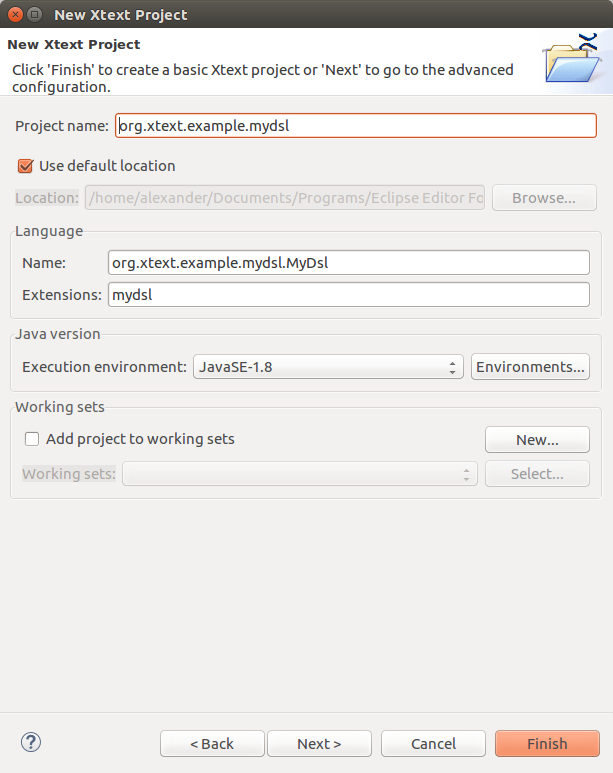
\includegraphics[width=\linewidth]{./Screenshots/newXtextProject.png}
    \caption{page 1}
  \end{subfigure}
  \begin{subfigure}[b]{0.45\linewidth}
    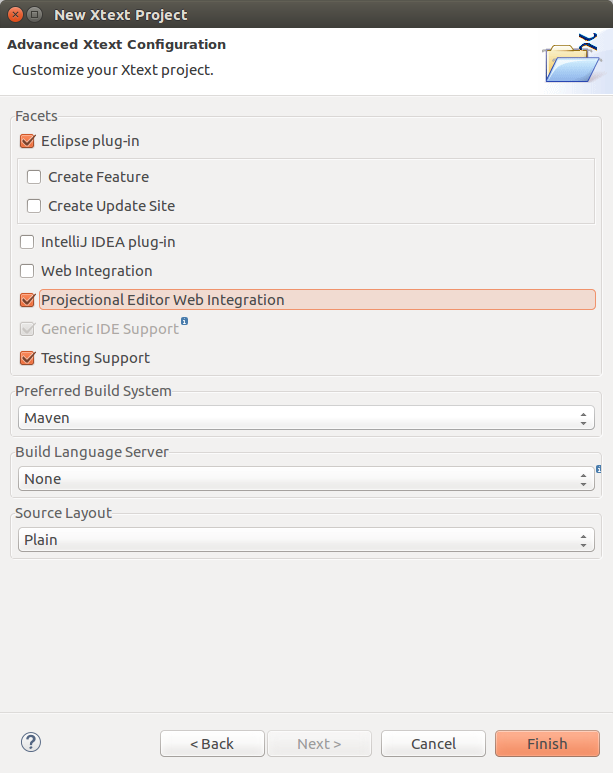
\includegraphics[width=\linewidth]{./Screenshots/newXtextProjectPage2.png}
    \caption{page 2}
  \end{subfigure}
  \caption{The modified "new xtext project" wizard}
  \label{fig:newProjectWiz}
\end{figure}
selecting the "Projectional Editor Web Integration" facet which has been added to the wizard next to the existing option for creating a textual web editor.
\\
\\
This creates an Xtext language project, shown in Figure
\begin{figure}[h!]
  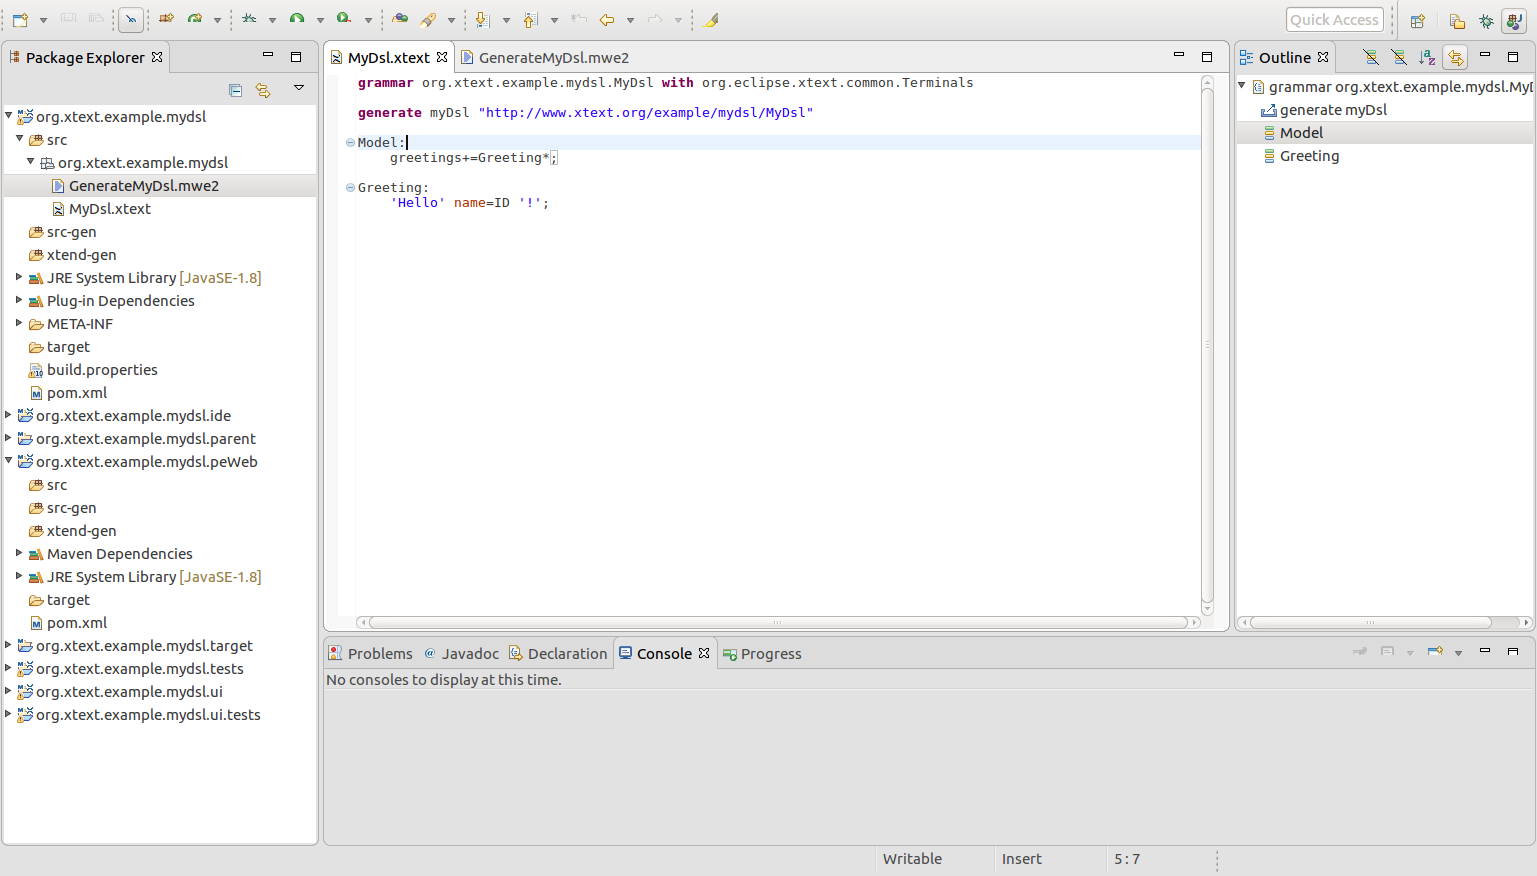
\includegraphics[width=\linewidth]{./Screenshots/newProjectScreen.png}
  \caption{A new xtext project with an empty peWeb project}
  \label{fig:newProjectScreen}
\end{figure} \ref{fig:newProjectScreen}, with a \emph{.xtext} file to specify the DSL's grammar and a \emph{.MWE2} file to describe the generation of the selected facets as usual. A number of empty projects are also created which will contain the files generated by the grammar definition. Notice the \emph{org.xtext.example.mydsl.peWeb} project which has been created and populated with a maven \emph{.pom} file which will be responsible for dependency management and has automatically been configured with the dependencies required by the projectional web editor. 
\\
\\
The generated MWE2 file for the language looks as follows:
\lstinputlisting[ tabsize=2 ]{Listings/GenerateMyDsl.mwe2}
It contains information on the language configuration and how facets for the language should be generated. As we selected the PE facet in the new project notice peWeb is enabled in this file. Because of this, when the user generates the language in the standard Xtext way, by running this MWE2 workflow file, the peWeb project will automatically be populated with all the necessary files to run a server for web based projectional editing. This results in the peWeb project looking like in Figure 
\begin{figure}[h!]
  \centering
  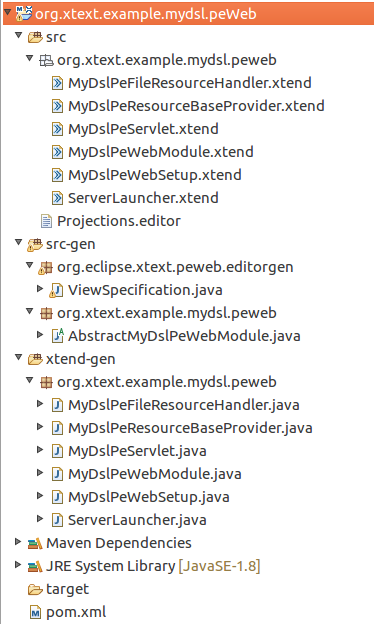
\includegraphics[width=0.4\linewidth]{./Screenshots/peWebProjectContentsAfterGeneration.png}
  \caption{The peweb project following generation}
  \label{fig:generatedPeWebProject}
\end{figure} \ref{fig:generatedPeWebProject}. Notice that MyDsl will be replaced with the name of the language.
The files generated are listed in Table \ref{Tab:generatedFiles}.
\begin{table}[h!]
\centering
\begin{tabular}{| m{7cm} | m{8cm} |}
\hline
File & Description \\
\hline \hline
Projections.editor & An empty file in which the language designer can specify the projections for the editor using the \emph{.editor} language discussed later.\\
\hline
MyDslPeServlet.xtend & A HTTP servlet which implements the projectional web API discussed later.\\
\hline
ServerLauncher.xtend & A servlet container to host MyDslPeWebServlet. When ran this starts the language server \\
\hline
MyDslPeFileResourceHandler.xtend & Allows the language designer to specify how files should be read or written, so that any persistence layer can be used. The generated file defaults to simply writing and reading files with the language's extension in the location given by  MyDslResourceBaseProvider \\
\hline
MyDslResourceBaseProvider.xtend & Used to specify how file URI's should be generated for a specified resource in the language. Defaults to a user-files folder at the location of the project.\\
\hline
MyDslPeWebModule.xtend & Allows binding of additional components in the language injector. This is where the resourceHandler and resourceBaseProviders are registered.\\
\hline
MyDslPeWebSetup.xtend & Creates the language injector itself, which will be used to inject information about the specified language into the otherwise generic language server implementation\\
\hline
\end{tabular}
\caption{Generated Files}
\label{Tab:generatedFiles}
\end{table}All of the generated files, with the exception of the \emph{Projections.editor} and \emph{MyDslPeServlet}, are required by Xtext's default textual web integration, and so will be familiar to existing XText users. One thing of note is that the FileResourceHandler and ResourceBaseProvider files are not automatically generated in the textual case but are still required. Here by assuming a simple implementation of saving to the local file system, we can generate these files automatically and so enable language designers to get a language server running much more quickly in order to test their language. In fact, at this point, the language designer simply points the serverLauncher to the location of a client application to host (we present a default such implementation in \ref{clientApp}), and the full web editor for their language is ready to run. There is no disadvantage to this generation as these files can be freely changed later or immediately.
%Maybe y generating like this at runtime we can use properties of the language. right now only name but could modify other things too.
%>Fact they are displayed to user means easily extensible matching requirement \RCustom
%>Talk about how the files generated are all commented (TODO) so clear what they are for and so easy to customise \RCustom
%\\
%\\
%\\
%\\
%\\
%\\
%\\
%\\ API
%\\
%\\
%\\
%\\
%\\
%\\
%\\
%\\
%\\
\section{Projectional Editor Web API}\label{api}
In this section I present the design of a server-side web API to allow a client to display and interact with projections for an arbitrary language. It is this API which the generated Projectional Language servers implement in my Xtext extension. It is important to note however that this API is dependent only on the general modelling assumptions I state in \ref{apiAssumptions}, and so is not tied to my Xtext extension and could be implemented by a server generated by any other language workbench or manually created for a general purpose language.

\subsection{Modelling Assumptions}\label{apiAssumptions}
\todo{Better to display this section in terms of a model diagram?}
As this API will be targeting arbitrary languages it is first important to make assumptions about the form of an AST within a programming language. To do this we studied the AST formalisms used by the three most popular language workbenches, given in Section~\ref{astFormalisms}, and ensured the model our API uses is consistent with these. We also make certain assumptions about the structure of a "project", or collection of files, within a language. The resulting modelling assumptions are:
\\
\\
\textbf{Programming Language Definition} = $\{\mathbb{T},\mathbb{D}\}$ 
\begin{itemize}
\item $\mathbb{T}$ - Node Types, a finite set of strings representing the different possible node types which may occur within an AST for the language.
\item $\mathbb{D}$ - Data Types, a finite set of strings representing the different primitive datatypes which may occur within an AST for the language. Note the assumption was made that values of these datatypes are all serialisable as strings, a fair assumption as most languages are entirely driven by the parsing of strings.
\end{itemize}
%
\textbf{Code Project Definition} = $\{n,F \}$ 
\begin{itemize}
\item $n$ - The name of the project as a string
\item $F$ - A set of files (definition below) which this project contains
\end{itemize}
%
\textbf{File Definition} = $\{n, L, a\}$ 
\begin{itemize}
\item $n$ - The name of the file as a string
\item $L=\{\mathbb{T},\mathbb{D}\}$ - The language to be used in this file
\item $a$ - An abstract syntax tree node for the language L which represents the root node of the AST in this file
\end{itemize}
%
Given a language definition $\{\mathbb{T},\mathbb{D}\}$ we define:\\
\\
\textbf{Abstract Syntax Tree Node Definition} = $\{t,C,R,A\}$ 
\begin{itemize}
\item $t\in \mathbb{T}$ - The type of this node in the language
\item $C$ - A finite set of references (definition below), the node's \emph{containment} references, that is the children nodes of this node which may not exist independently of this node. An example in a general purpose language might be a reference to an Expression node from within an If Statement node.
\item $R$ - A finite set of references (definition below), the node's \emph{cross} references, that is references to other nodes which exist independently of this node. An example in a general purpose language may be a Function Call node may cross reference a Function Definition node.
\item $A$ - A finite set of attributes (definition below), the actual data of the node.
\end{itemize}
%
\textbf{Reference Definition} = $\{n,t,R\}$ 
\begin{itemize}
\item $n$ - A string giving the name of this reference.
\item $t\in \mathbb{T}$ - The node type of the nodes being referenced 
\item $R$ - A finite list of AST nodes such that $\{t',C',R',A'\} \in R \implies t'=t$
\end{itemize}
%
\textbf{Attribute Definition} = $\{n,d,A\}$ 
\begin{itemize}
\item $n$ - A string giving the name of this attribute
\item $d\in \mathbb{D}$ - The datatype for the value stored in this attribute
\item $v$ - A value from the datatype $d$
\end{itemize}
%
\subsection{Design}\label{apiDesign}
I now discuss the design of the API itself, giving it's full specification in the appendix. When designing this API it was necessary to consider the relevant requirements for the project's ultimate goal as given in \ref{requirements}. The requirements to produce a lightweight (\RLightweight) and customisable (\RCustom) editor are clearly relevant here.
\\
\\
The first consideration was how best to transport the state of the abstract syntax tree between client and server. Existing solutions in textual web editing, such as within LSP or Xtext's own default web editor implementation rely on first synchronising the client with the server by sending the full contents of a document as a string. Further requests or edits are then handled by referencing positions within the document as line/position numbers or ranges. This pattern of synchronisation followed by incremental updates between client and server has the advantage of minimising the data transmitted. In order to do this on ASTs directly however, we need some way of referencing nodes within a tree. We achieve this by annotating each node within an AST on the server side with a unique identifier. If the client is then aware of this labelling we can use it to communicate incremental changes between client and server, such as changes to attribute values.
\\
\\
Having decided upon this annotation of the ASTs in order to reference incremental updates, we next look at the initial synchronization. In order to keep the client application as lightweight as possible (as per \RLightweight) we wish to minimise the data synchronised onto the client. We notice that the client only ever needs to maintain state relating to the parts of the AST(s) that they are actively interacting with. With a textual representation, this is very difficult to determine, and by default we assume the user wishes to display the entire textual contents of a file. However, a projectional editor has no such issue. At any given time a user is interacting only with projections of the AST, these projections define explicitly which nodes of the AST, and which attributes within these, are relevant and should be displayed. Hence we have no need to synchronise all details of the AST with the client initially, only as and when these are required by a projection.
\\
\\
With this in mind then, initial synchronisation happens as follows. Upon opening a file the client application requests a "skeleton" tree, consisting only of node names (generated by the language server, using certain attribute values or the node's type) and their unique identifiers. This can be used for navigation within the file, enabling the user to request projections for subtrees they wish to edit instead of for the whole file. Through some means then, a subtree is selected to be displayed, the client makes a request to fetch that subtree's root node using the ID from the client's skeleton tree, and the server responds with the attributes and references which will be displayed within the projection for that node in some format. From here we are ready to begin transmitting only incremental changes made within this projection between client and server. In the case that the user wishes to edit a different subtree we can then ask for the values relevant to that node using it's ID from the skeleton tree which we can keep cached.
\todo{Include a diagram here}

\subsubsection{Transferring Node State}\label{apiNodeStateTransfer}
To actually display and interact with an AST, the client needs both information about the current state of the relevant nodes, and how to project this state. There are two approaches to doing this which place different requirements on the client.
\begin{enumerate}
\item Require the client application has definitions for the possible projections, so given the state of a node, and the name of the projection to use, the client can create the projection itself.
\item Information about the projection should be sent along with the state of the node, then the client need not know anything about the language or projections at compile time, as these are supplied by the language server.
\end{enumerate}
Both approaches have advantages, the first allows for more flexibility in the projections that can be written, and if a projection is to be used by many nodes reduces the amount of data to be retrieved from the language server. The second approach however keeps the size of the client application much smaller, especially if the language is large and requires many different projection types. Since projection specification is inherently associated with a language, it is also the case that only the second approach allows a client application to remain language independent while still being able to display language specific projections.
\\
\\
Because both have advantages, in line with our \RCustom requirement to allow as much flexibility as possible for language designers, we decide to design this API such that both approaches are possible.
\\
\\
To achieve this the API specifies that a node fetch response should simply be as an arbitrary JSON~\cite{json} object with a type field. The client should be capable of decoding the object based upon it's type. We make use of two language independent node-fetch types in this project which can be assumed to be standard, and should prove sufficient for most use cases. Language designers can still however create new node-fetch types for the language server to use, provided they extend the client application accordingly to handle these new types. 
\\
\\
The two standard types are:
\begin{itemize}
\item \emph{Default Projection}: The client is given all the attributes and references for the node which it then presents to the user in any meaningful way as decided by the client application.
\item \emph{CustomHtml Projection}: This method involves sending not only relevant attributes for the node to the client, but also sending HTML to specify how it should be projected. The intention is that these will be automatically generated by the projection specification language given in Section \ref{EditorLanguage}.
\end{itemize}
We discuss these in more detail in Section \ref{viewObject}.
\subsubsection{Making Changes to a Node}

We notice from our modelling assumptions that a node consists of a series of attributes, \textit{containment} reference features and \textit{cross-reference} reference features. In order to make changes to nodes we thus provide 3 methods in our API to modify these. Each method takes as parameter the project name, file name and nodeId of the node being modified so that the server doesn't have to store state regarding which nodes clients have requested and are editing. The methods are as follows: 
\begin{itemize}
\item \emph{update-attribute} : Takes the attribute name  of the node and it's new value (as a string, using our assumption here that all datatypes in a language are serializable as such). 
\item \emph{add-reference} : Takes the reference feature name as a parameter. In the case of a cross-reference we also expect a child-id parameter, that is, the identifier of the node we wish to cross reference. The language server then adds this reference. In the case of a containment reference no additional parameters are required and the language server creates a new node of the type specified by the reference feature's type. The language server assigns this a fresh identifier and sends the skeleton subtree rooted at this new node back to the client so it may update it's skeleton tree. (This response allows the language server to create children for the newly created node if required as a side-effect)
\item \emph{remove-reference} : Takes the reference feature name and ID of the node to remove as parameter. It then removes the reference from the feature, and if it was a part of a containment reference then it deletes the node from the tree and removes all cross references to it from other nodes.
\end{itemize} 
%\\
%\\
Following the update of a node we can check that we have left it in a valid state using the \emph{validate-node} method which takes as parameter the project name, file name and nodeId of a node and returns an object which either signals that the node is in a valid state OR that it isn't and a string with the error message. In the case of removing a containment reference, as other nodes may have cross referenced it, we must instead use the \emph{validate} method, which will return a list of every node which is not in a valid state with the matching error strings.

\subsection{Implementation in Xtext}
I now explain how this API is implemented in the automatically generated language servers from my Xtext extension.
\\
\\
The generated server hosts a Java HTTP servlet. In order to make API calls the client is expected to send get requests to the url pattern specified by the language designer in the generated \emph{MyDslPeServlet.xtend} file, which, by default, is /pe-service/. The client uses a http parameter serviceType to choose the API call to make, and adds other parameters to the request as required by the API call made. The server responds with standard http error codes if there is a mistake with the request parameters or in the execution of the method or otherwise with a JSON object containing the response of the call.
\\
\\
In order to get files and project details, the language server injects the FileResourceHandler and ResourceBaseProvider objects specified in the \emph{MyDslPeFileResourceHandler.xtend} and \emph{MyDslResourceBaseProvider.xtend} files. These objects define operations to get and save EMF resources from a "resource id" (we use PROJECTNAME/FILENAME) so that arbitrary persistence layers can be used. By default these correspond to storing files in their textual representation at /user-files/PROJECT_NAME/FILE_NAME.LANGUAGE_EXTENSION relative to the language server, so that loading a file is equivalent to parsing the stored textual representation into an AST, and saving uses the parser rules to create a textual representation from the AST. Retrieving a file using the method in the FileResourceHandler results in an EMF Resource object, from which we can retrieve the EObject which represents the root node of the AST that file represents.
\\
\\
The EObject retrieved closely matches an AST as we described in our modelling assumptions, containing reference features linking to other EObjects and attributes. When we first open a file and retrieve it's EObject all that remains then is to annotate the tree with unique identifiers as discussed in \ref{apiDesign} which we do recursively from the root. We also construct two additional maps, one from these identifiers to the respective annotated node, and another from the EObjects themselves to the nodeIds. The first of these maps allows us to efficiently find nodes referenced by API calls, the second allows us to find the nodeId of a node even if we obtain it by following the unannotated EObject's references directly. These maps are kept up to date incrementally as nodes are added and removed from the tree.
\\
\\
Modifying nodes is then done by looking up the relevant node using the nodeID to EObject map and then making the relevant changes to the EObject itself.
%EObject contains all the attributes and reference types as well as some constraints on the node so already have AST in effect
%From these nodes we create a tree where children of a node are all those contained only in containment references, that is every node is only in this tree once
%We annotate it with node identifiers which we do when we first open the file
%We also create a map from these  nodeIds to the EObjects themselves
%We also create a map in the other direction, so if we follow a reference in the EObject we can easily look up the node ID if we need to communicate this with the client
%This is all cached and kept up to date incrementally as the tree changes
%Modifying nodes is all done by looking up the nodes with the nodeId-> eobject map and then modifying the eobject directly
%\\
%\\
%\\
%\\
%\\
% Editor Language
%\\
%\\
%\\
%\\
%\\
%\\
%\\
%\\
%\\
%\\

\section{Projection Specification Language}\label{EditorLanguage}
\subsection{Overview}
The real power of a projectional editor lies in it's ability to allow a user to interact with a programming language in an intuitive way using projections that are designed alongside the language. In this section I present a DSL developed to rapidly specify custom projections for ASTs of an arbitrary language. We use this in our Xtext extension to allow language designers to create such specifications for their own languages, however, like the API discussed in Section \ref{api}, this language was designed independently of the Xtext extension, and so could be used within other language workbenches.
%Ultimately the goal being to provide a standard way for language designers to define projections for their language within a language workbench which can then be used in the automatic generation of a web projectional editor.
\\
\\
The relevant requirements from Section \ref{requirements} are \RSetup (ease of setup), \RCustom (customisability), and \RFamiliarity (familiarity). Specifically in this context that translates to ensuring that the designed language is simple and easy to use, requiring as little time as possible to learn. The language should also be as powerful and flexible as possible in terms of the projections it can define.

\subsection{Design}

It seemed clear that using a combination of HTML and JavaScript to specify projections would be the most natural thing to do. The HTML can then be sent to the user and displayed within the client application. Depending on the implementation, this approach could allow much flexibility, as HTML and JavaScript themselves do, while also keeping the proprietary part of the editor specification language smaller. Both of which align with our requirements. For further inspiration we looked at MPS's editor specification language.

\subsubsection{MPS Editor Language}
The MPS language workbench has it's own editor language~\cite{mpsEditorLanguage} which is used to specify projections for a language's "concepts" (their term for our nodes). The language works simply as follows: For each concept a user uses cells to build up the look of the projection. These cells may contain the following:
\begin{enumerate}
\item Constant cell - Displays a constant string value
\item Collection cells - containers for more cells to build up further structure
\item Property cell - Space to display and edit attributes textually
\item Child cells - to display the projection of a child
\item Referent cells - to display a custom view of a child
\item Child List cell - as per child cell but displays all children of the same type, allowing the user to customise how they are separated etc.
\item Indentation cells - empty space, different from constant cell only in that indent size is managed by global editor settings
\item UI Component cell - holds a custom UI JComponent written by the language desinger, doesn't store state
\item Model access - allows custom access to an attribute of a node, the language designer specifies a get, set and validate method indicating how the cell should reflect the node's attribute and how changes to the cell should set the relevant attribute. Validate gives a boolean function indicating whether or not the node is in a valid configuration.
\item Custom cell - the language designer can create a custom cell by implementing the EditorCell interface in MPS
\end{enumerate}
%
We allow this to inform the design of our own language as follows. First we notice that most of the cells are used to control the layout of the editor, we can use HTML for this purpose and so can ignore these cells. The remaining functionality this language offers then is:
\begin{enumerate}
\item Properties/Attribute access - Some way to access the attributes of a node, displaying them to the user and allowing them to edit them.  (Covering here the Property cells and Model Access cells)
\item Reference access - Some way to specify where a node's children (references) are displayed, and specifying how they should be displayed (as per the Child, Child List and Referent cells of MPS)
\end{enumerate}
Using MPS's idea of placeholder cells, we decide to augment HTML with additional tags which will, like the cells in MPS, be replaced at runtime with the relevant HTML to display attributes or projections of child node. With regards to the placeholder cells in MPS, one nice feature is the ability to customise how these actually appear, with attributes we can use "Model Access" cells to completely customise how a user interacts with the attribute and similarly with "referent" cells the language designer can define different projections to display child nodes from within another projection. This functionality aligns with our goal to ensure our language is as flexible as possible, and so we will attempt to give similar functionality to our own language.

\subsection{Language Specification}
I will now give a brief overview of the editor language specification, before presenting it in full and then covering important aspects in greater detail. 
\\
\\
The editor language allows the language designer to specify one or more named projections for each node type, using HTML to describe the layout and JavaScript to describe how the projection should be populated with the node's attributes and how to detect edits to these. If a node contains references to other nodes, these can be inserted into the projection by means of additional annotations within the HTML, which will be replaced with projections for the referenced nodes. The language also allows the declaration of components which represent reusable pieces of a projection which may be used across different projections to allow code reusability. 
\\
\\
The complete specification for the language follows, using extended BNF with the addition of the standard regular expression symbols *,?,+ for succinctness. I will then discuss the different parts of the language in more detail.

\setlength{\grammarparsep}{12pt plus 1pt minus 1pt} % increase separation between rules
\setlength{\grammarindent}{5em} % increase separation between LHS/RHS 

\begin{grammar}

<EditorDefinitionFile> ::= <ImportSection>? <MainSection>

<ImportSection> ::= (`import' <QualifiedName> `;')+ 

<MainSection> ::= (<NodeDeclaration> | <ComponentDeclaration>)*

<NodeDeclaration> ::= `Node' <ID> `{' (<ProjectionDeclaration> | <ComponentDeclaration>)* `}'

<ProjectionDeclaration> ::= `Projection' <ID> \\ `{ view:' <HtmlSnippet> (<AttributeDeclaration> | <ComponentDeclaration>)* `}'

<AttributeDeclaration> ::= `@'<ID> <AttributeController>

<AttributeController> ::= `{' `get:'<JSSnippet> `set:'<JSSnippet> `validate:'<JSSnippet> `}'

<ComponentDeclaration> ::= `Component' <ID> \\`{' `view:' <HtmlSnippet> <ComponentController>? `}'

<ComponentController> ::= `get:'<JSSnippet> `set:'<JSSnippet> `validate:'<JSSnippet> 
 
<ChildId> ::= `!' <ID> `:' <ID> `!'
 
<ComponentId> ::= `\%'<ID> (`:'<ID>)? `\%'

<TagId> ::= `\$' <ID> `\$' 

<HtmlAnnotation> ::= `<<' (<TagId> |<ChildId>|<ComponentId>) `>>'

<Js	Annotation> ::= `<<' <TagId> `>>'

<HtmlSnippet> ::= `['<CodeLiteral>`]'
\alt `['<CodeLiteral> <HtmlAnnotation> (<CodeLiteral> <HtmlAnnotation>)*  <CodeLiteral> `]'

<JSSnippet> ::= `['<CodeLiteral>`]'
\alt `[' <CodeLiteral> <JSAnnotation> (<CodeLiteral> <JSAnnotation>)*  <CodeLiteral> `]'
%\alt `for' <ident> `=' <expr> `to' <expr> `do' <statement> 
%\alt `{' <stat-list> `}' 
%\alt <empty> 

%<stat-list> ::= <statement> `;' <stat-list> | <statement> 

\end{grammar}

\emph{Note}: Terminal rules for CodeLiteral and ID have been omitted for the sake of brevity.

\subsubsection{Example}
Here is an example specification of a simple layout.

\todo{Add example file here, maybe for questionnaire? Needed?}

\subsubsection{Node}

Most files will consist primarily of node declarations. A node declaration should be included in the file for every node of the language for which custom projections are desired. To reduce the amount of work required on the language designers part, if a node is not found then this instead indicates some default projection should be used.  
\\
\\
A declaration can contain definitions of different projections for the node and also components which can be used only in the scope of this node.

\subsubsection{Projection}
Projection declarations exist within a Node declaration. Each projection declaration is named and specifies a way in which this node type can be viewed and controlled.
\\
\\
Multiple projections can be defined for a single node. When referencing children etc we can then specify which projection we retrieve using it's name. This is similar to the referant cell behaviour of MPS, but our approach, having named the projection and defining it as a part of the node type being referenced, allows us to reuse this view from within other nodes, making this method preferable.
\\
\\
The body of a projection declaration contains a view, and optionally, attribute controllers and component declarations.
\\
\\
The view attribute defines how the projection should look on screen. This is achieved using a HTML snippet delimited by square brackets. \todo{Square braces don't make sense for JS, should change this if have time} These HTML snippets can also include the following additional annotations:
\begin{itemize}
\item <<!CHILDNAME:PROJECTION\_NAME!>> : Indicates the reference with the name CHILDNAME should have its PROJECTION\_NAME projection inserted here. Used as the child node cells are in MPS. If the reference feature references multiple nodes then some default list view will show the set of children, each using the specified projection. Unlike in MPS I am not allowing customisation of the list layout itself at present, but this is a clear target for the future given more time.
\item <<\%COMPONENTNAME \%>> : Inserts the component COMPONENTNAME, enabling reuse of code.
\item <<\%COMPONENTNAME:ATTRIBUTE\_NAME \%>> : As above but if the component has an attribute controller (see below) attached to it then it uses this to populate the nodes attribute ATTRIBUTE\_NAME
\item <<\$ID\$>>: This tag is used to indicate an Id property of a HTML element. HTML elements must have unique id's and so we must assign them dynamically.
\end{itemize}

\subsubsection{Component}


A component looks similar to a  Projection with an optional attribute controller, and may be declared globally or within a node so as to allow code reuse.
\\
\\
The purpose of components is to allow for code reuse for common functionality such as text boxes for custom datatypes etc.
\\
\\
The import section at the start of the file allows the user to be able to import files containing default or third party components such as textboxes for ints, strings etc. so as to reduce the amount of code the user must write. 
%COMPONENT_NAME%{
%	view:[ ANNOTATED_HTML ]
%	(get:[ ANNOTATED_JS ]
%	 set:[ ANNOTATED_JS ]
%	 validate:[ ANNOTATED_JS ] )?
%}

\subsubsection{Attribute Controller}

An attribute controller dictates how an attribute's value should be get and set within the projection. A controller also allows a local validation function which can also modify the view if an input is invalid/valid. This is all achieved using JavaScript snippets with additional <<\$ID\$>> annotations to reference elements specified in the view.
\\
\\
An attribute controller has three methods, get, set, and validate. Get expects a js snippet which evaluates to a string e.g. it retrieves the value of the attribute from the projection/component. Set expects a js snippet which will be executed in an environment where the value of the attribute is assigned to the variable X, this can then be used to initialise attribute values in the view. Validate expects a js snippet which will be executed in an environment where the value of the attribute is assigned to X also and should evaluate to either true or false to indicate whether or not this is a valid value. 
\\
\\
For example a simple text box: 
\lstinputlisting[tabsize=2]{Listings/TextBox.editor}
This component can then be placed in a projection and assigned to control the value of an attribute for the projected node.

\subsection{Implementation}
The \emph{.editor} language was implemented using the standard version of the language workbench Xtext. This involved specifying the language's grammar in Xtext's grammar specification language, (given in the appendix \ref{editorLanguageGrammar}), and also specifying the compilation process for the language. The result is a plugin for both Eclipse and Intellij which includes an editor for the language complete with syntax highlighting, context completion etc. making writing a \emph{.editor} file much easier. The \emph{.editor} language compiles into a java representation of itself which can then be used by the language server to create view objects to send to the client application.
\\
\\
With regards to our final tool, we have taken the generated \emph{.editor} Eclipse plugin and merged this with the main Xtext plugin. This means that our extended Xtext plugin provides syntax highlighting, context hints etc. for \emph{.editor} files directly, and also automatically compiles these into their java representation to be used by the language server at runtime.
\todo{screenshot here of syntax highlighting?}
\todo{More explanation about how generated?}

\section{Fetching Node State}\label{viewObject}

Having discussed the \emph{.editor} language it is now worth discussing how this is used by the extension to send information about a node's state to a client using the get-node API call as was touched upon in \ref{apiNodeStateTransfer}. 
\\
\\
When a node is retrieved the server looks to see if a main projection is specified for the node in the java representation of the \emph{.editor} file which is generated automatically by the plugin. If so, we use the current state of the node requested and it's children to recursively build a custom view object with the following signature which we then send to the client application:
\lstinputlisting[language=TypeScript, tabsize=2 ]{Listings/custom-view-descriptor.ts}
%Listing
%Explain Listing ?
\todo{Needs more description here?}
If a node doesn't contain a main projection we instead create and send a default projection with the following specification: 
\lstinputlisting[language=TypeScript, tabsize=2 ]{Listings/default-view-descriptor.ts}
This allows the language designer to save time as they can run the editor application without having to specify any projections at all, or just customise projections for some select nodes. 
%Explain listing


\section{Client Application}\label{clientApp}
Here I present an implementation of a client application, written using the Angular framework, for use with a language server implementing the API from Section \ref{api}. This application serves as the default front end for a projectional web based editing application which has automatically been generated using our extension to Xtext language workbench. I also make much use of it to evaluate both the specified API and Projection Specification Language. 

\subsection{Design}
The client application was designed to offer a simple interface with all default functionality, that is primarily  supporting both Default and Custom view types as discussed earlier. The application was written using the Angular framework and typescript, as this offered all the features needed and is very popular. This means plenty of documentation is available and it should be easy for language designers to extend.
\\
\\
Extensibility was in fact one of the biggest considerations when writing this application. As this will be the UI with which a language's end users directly interact with, we expect a language designer will want to make changes to match their companies/institutions styling and also to build in other  deployment dependent features, like user authentication or training materials etc. To this end, the application is built in a very modular fashion, so that it is easy to modify and extend. This was easy to achieve using Angular components and services. Notably, all interaction with the language server via the API is written as a separate service which maybe imported into a different application implementation. Likewise the actual display and editing of a node via a projection is a separate component, and so the language designer may easily import and place this anywhere within a different client application.
\subsubsection{UI}
The UI takes some inspiration from the online IDE Theia~\cite{theia} with navigation all happening on the left hand side leaving a large space for the projections on the right. The intention was for this default UI to be as simple and clean as possible, so that it if a language designer doesn't require additional features or require specific styling the default UI should be appropriate. It was also designed to be easy to use by end users. These two considerations reflect requirements \RSetup and \RIntuitive respectively.
\begin{figure}[h!]
  \centering
  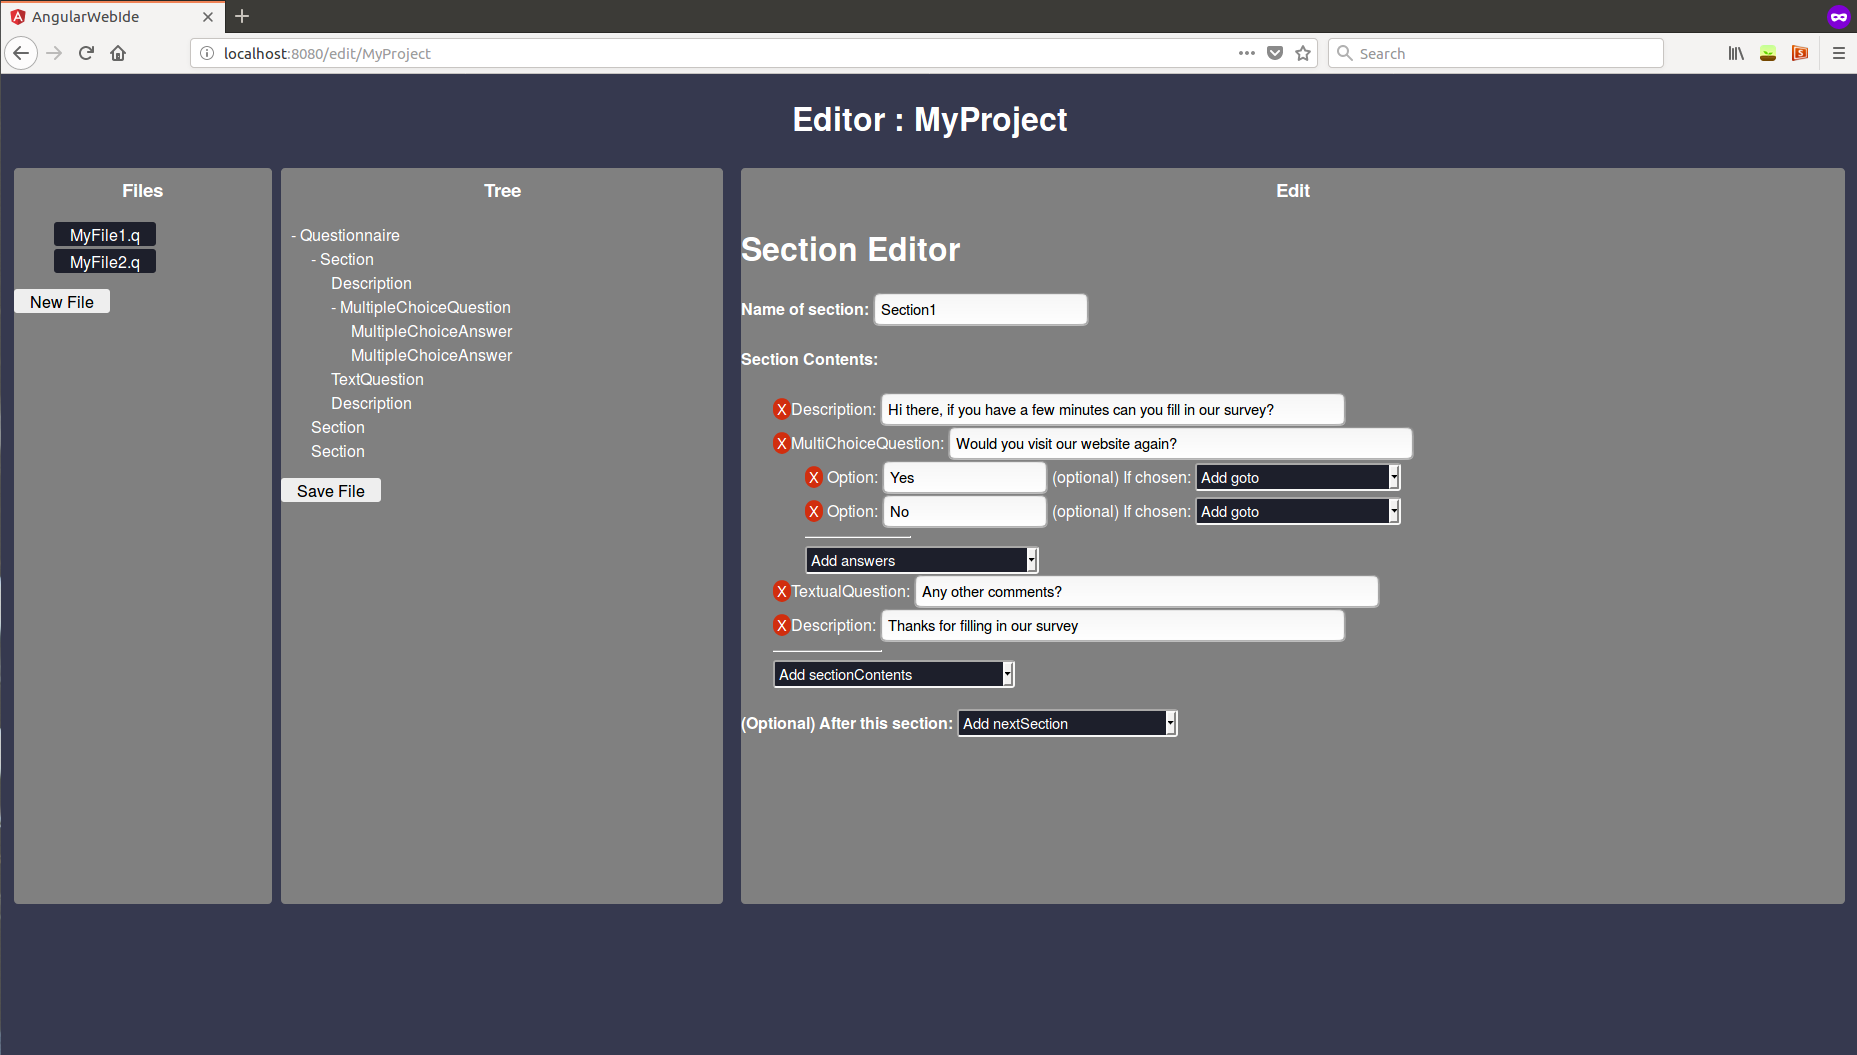
\includegraphics[width=\linewidth]{./Screenshots/WebUIScreenshot.png}
  \caption{Editing the questionnaire language from \ref{questionnaireLang} in the default client application}
  \label{fig:webUI}
\end{figure}
%
%\subsection{View Implementation}
%
\todo{Discuss implementation of views here?}
%>Asynchronous calls, separating services and response code to separate concerns so easy to make new UI as desired
%>Discuss 2 kinds of view and implementation
%>Evaluate Performance
\section{Evaluation}\label{evaluation}
In order to evaluate the work of this project I focus on two areas. The first is on the process of language creation and the flexibility of the tool presented as a method for creating projectional editors for arbitrary languages. The second area looks at the ability of the tool to address the problem laid out in Section \ref{problem}, that is, the ability of an editor produced using my tool to improve accessibility of a DSL to a non-technical audience.
%\\
%\\
\subsection{Projectional Editor Creation}\label{creationEvaluation}
In order to evaluate the projectional editor creation process I built three 3 languages and comment here on the process. The three languages are as follows:
\begin{itemize}
\item An expression language to define mathematical functions using the usual 4 binomial operators and a summation function.
\item A DSL for specifying the content and flow of questionnaires
\item A subset of the language Pascal as presented in the Compilers course which has been extended with the addition of node graph primitives. 
\end{itemize}
%
\subsubsection{Expression Language}
The expression language allows a user to define mathematical functions on variables using the 4 usual binary operations and a summation function. The intention was to test the ability of the editor language to produce a projection which resembles written mathematics.
\\
\\
The creation process for this language was fairly straightforward, the only required code being the standard grammar file and \emph{.editor} file to specify projections. I found the process of writing the projections simple for all nodes bar the creation  of the summation and division nodes which required the use of HTML tables to correctly format to mimic the look of natural mathematics. The difficulty in doing this was in using the correct HTML align attributes without any visual clues. In order to get the positioning just right I found the best thing to do was to use the HTML inspector in my browser, modify the alignment values and then copy these back into the editor file. This clearly indicates that the \emph{.editor} file editor could be improved by some ability to peek at the projections as they are being written. A projectional editor for the language could do exactly that, and so it may be interesting to try and re-implement this language within the tool I have created.   
\\
\\
Another finding here is that the buttons to remove nodes can be visually distracting, and so it may be worthwhile looking into alternate ways this functionality can be achieved. A contextual menu is an obvious choice but really we would want this to be customisable. In order to do this it might be worth extending the language so that the language designer can write reference controllers in a similar vein to the attribute controllers, writing arbitrary JavaScript to specify when nodes should be removed or added.
\begin{figure}[h!]
  \centering
  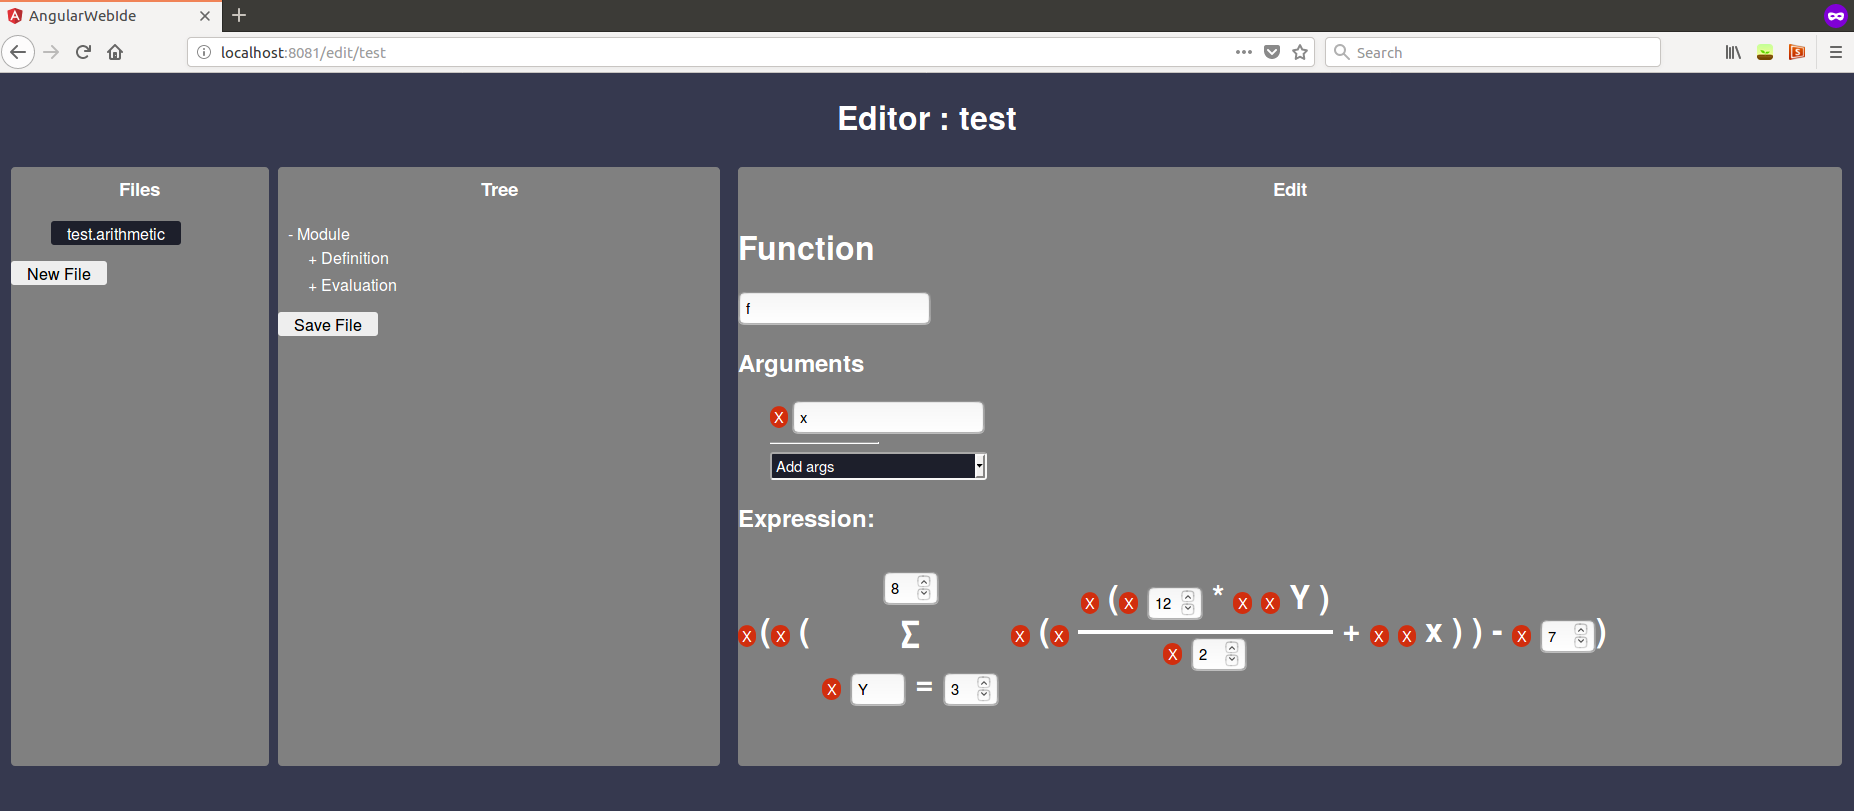
\includegraphics[width=\linewidth]{./Screenshots/arithmeticUI.png}
  \caption{The expression language editor}
  \label{fig:arithmeticUI}
\end{figure}


%To Add Grammar Definition (In appendix)
%To Add Projection file (in appendix?)
%Screenshots of projections

%Process: Just modified projections file
%Findings: Two step process, only new step as language designer is to create editor language file found this a little fiddly without a HTML viewer as trying to adjust HTML table difficult. This could be massively improved with a view component for the language, an obvious extension for this language would be to create a projectional editor to do exactly that, so always displaying what result would look like. 
%Having delete circles breaks illusion of 
\subsubsection{Questionnaire Language}\label{questionnaireLang}
A language to be used to specify questionnaires consisting of multiple pages containing text (titles and descriptions) and questions (textual and multiple choice). Flow of a questionnaire can be controlled by referencing other sections and using basic branching on multiple choice answers. This language is used in the second section to evaluate the accessibility of projectional editors created with my extension in comparison to textual ones.
\\
\\
The creation process for this language was much easier than for the expression language. Again only the standard grammar and projection files were required, however the projection file was much easier to write as there was no intricate positioning to worry about. The created editor seemed very usable and, as the language has a much smaller tree depth than the expression language, was not marred by the default reference layout with buttons and dropdowns, in fact here they seem to be the obvious choice. This confirms that these should not be changed to another default layout but the language should be extended to allow customisation of these in some way.

%Grammar Definition In appendix
%Projection file (in appendix?)
%Screenshots of projections

%Process: Modified Projections file
%Findings: This is clearly where the projectional editor shines, very easy to define for a specification language as projections were not as fiddly as in the previous case. Also resultant editor seems more useful as not having large tree depth as in expression language.


\subsubsection{PasGraph Language}\label{pasgraph}
This language is a subset of the programming language Pascal~\cite{pascal}, that has been extended with: 
\begin{itemize}
\item Node graph primitives
\item Particle primitives which are defined on vertices upon said graphs
\item A move statement which moves a particle to a randomly connected vertex
\item A binary relation, a ->-> b to test if a and b are on the same graph and if so whether or not b is reachable from a.
\end{itemize}
This language could perhaps be used to simulate the coalescing of particles performing random walks on graphs for example. 
\\
\\
The language was designed and chosen to evaluate the performance of web editor generation on a general purpose language, and also to evaluate the flexibility of the possible projections, node graphs having a clear non-textual visual representation which we would like to use.
\\
\\
The process for creating the editor was slightly more involved than the other two as we wanted to use the d3 JavaScript library~\cite{d3} to display and edit the node graph primitives. In order to achieve this we had to override the standard ViewRetriever object which is responsible for creating the view objects sent as response to get-node requests (as discussed in \ref{viewObject}). We add a check to see if the tree node requested is a node graph, and if so return a special view object with the type "NodeGraph", listing the vertices and edges of the graph in a form that d3 can plot. A single line was then changed in the generated GraphPeServlet file to make use of this.
\\
\\
\begin{figure}[h!]
  \centering
  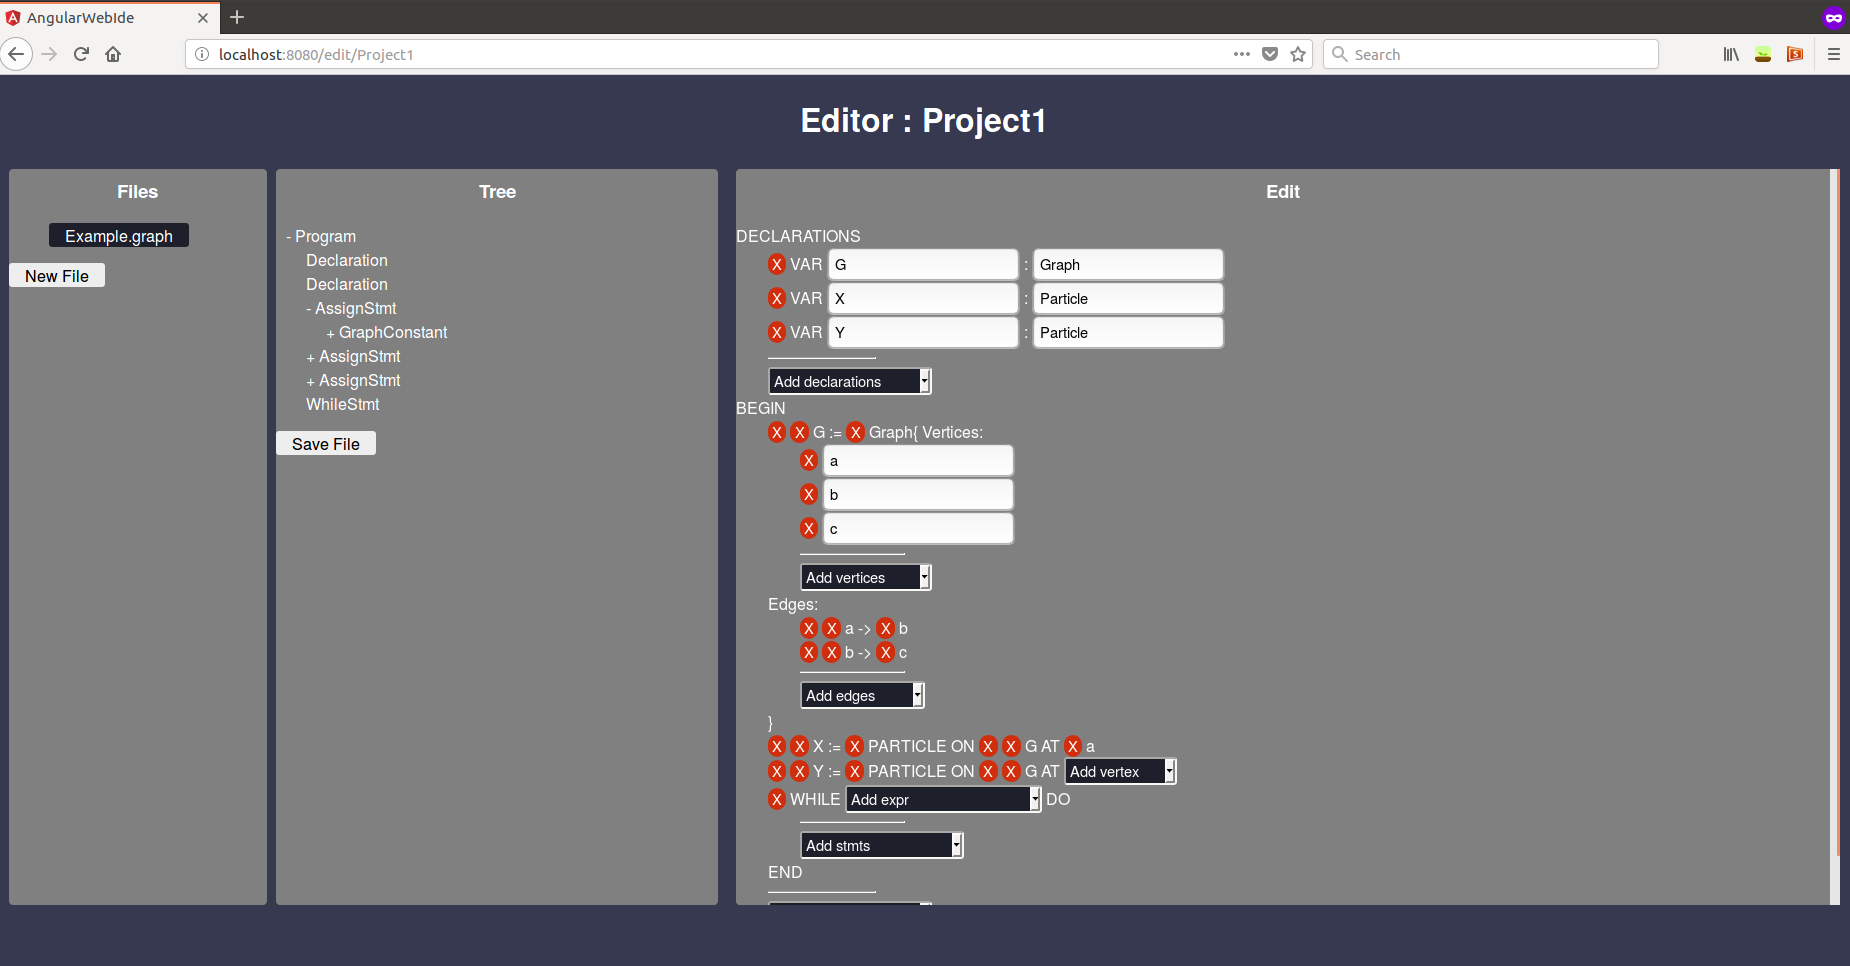
\includegraphics[width=\linewidth]{./Screenshots/graphUI1.png}
  \caption{The PasGraph language editor displaying several statements}
  \label{fig:pasgraphUI1}
\end{figure}
\begin{figure}[h!]
  \centering
  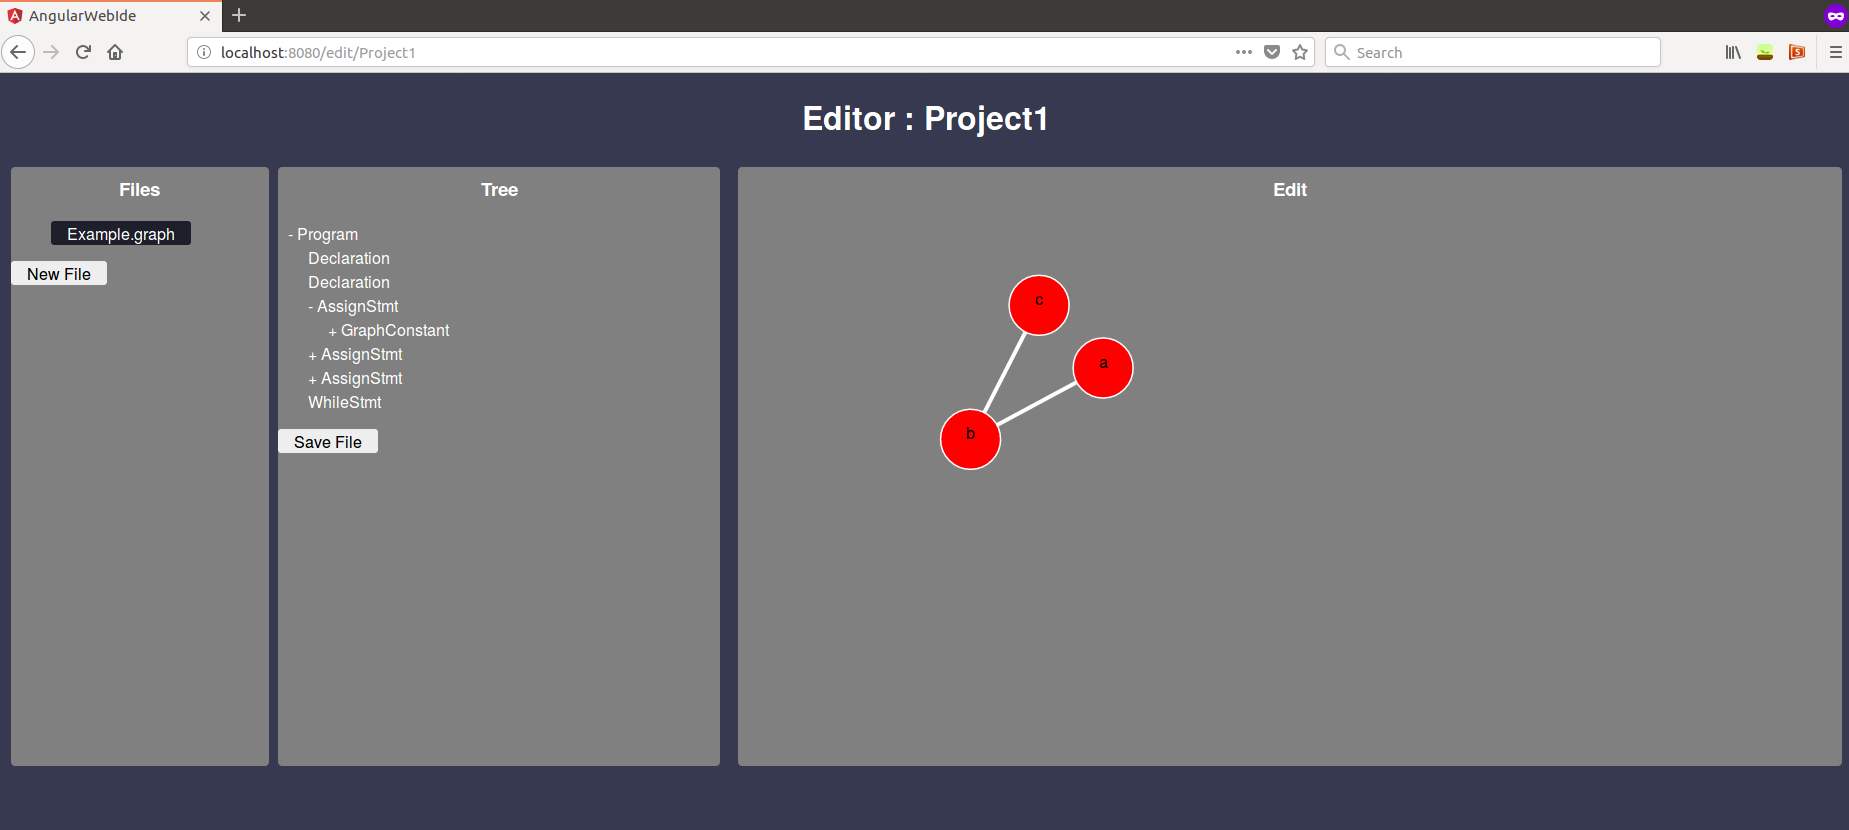
\includegraphics[width=\linewidth]{./Screenshots/graphUI2.png}
  \caption{The PasGraph language editor projecting a graph constant}
  \label{fig:pasgraphUI2}
\end{figure}
The front end was then modified with the addition of a self contained component which, when given a NodeGraph view object, would plot the graph using a d3 force simulation and allow a user to interact with it. Using the edit service it was easy to allow interaction with this graph to update the abstract syntax tree, for example when the user clicks in an empty space, a add-reference request is sent to the server to create a vertex child, and upon receiving a success response a vertex is then added to that location in the diagram. The only other required change in the front end was to add the NodeGraph case in the main editor component which chooses which component to use based on the type of a get-node response.
\\
\\
All in all the creation of the language was still very straightforward, almost all of the additional code required for the complex projection required being written in entirely separate components which were then easy to integrate with the existing code. The remaining projections were created using the editor language as normal and so as a whole the editor creation process was still fairly quick. This demonstrates that the extension has very successfully achieved \RSetup and \RCustom, the tool allowing very quick specification of nodes with non-interesting projections but allowing arbitrary web technologies to create more complex projections when required. Crucially it also allows this in a way that such complex projections require little work to integrate with the generated editor. 
\\
\\
The method used here also indicates an advantage that these web projectional editors have over their non-web-based projectional counterparts. In the graph node example we send to the front end a list of vertices and edges which are then displayed, but we could have sent anything we'd wanted. If the projection we desired were more complex, say including a 3D view of some simulation, we could have exploited this behaviour to have the server conduct any expensive calculations/preprocessing required by the projection and sent this within the view object. This could substantially reduce the hardware requirements for the final developer's machine if complex projections are required.
\\
\\
One issue noticed in the implementation of this language is that new projection types cannot be mixed with those specified in the \emph{.editor} file. This means that the visual projection of the graph could only be used when editing the graph in isolation of the rest of the tree, and at other times a textual representation was required. However this could easily be solved by modifying the protocol for getting a node, so that instead of asking for and expecting a single view object containing all projection information of the children, the client must recursively ask for these, enabling it to display children using different front end components.
%
%
%Screenshots of projections
%Findings: Easy to modify projections for all standard language constructs. Added extra projection view for graph and this process was easy as could extend viewRetriever etc. Default projections were not suitable for this language as makes sense to make them look like the textual representation. Custom view objects constructed before being sent, found issue with this as couldn't include other projection types within a customHTML view so graph editor had to be on  separate page, would want to change this so the client recursively called the get-node. This would also have the advantage of allowing default projections to be sent within custom nodes
%Way language defined does now have impact on editor, moreso than with textual editor. For Example compare way expressions are defined in this vs Expression language. This has the operation as an attribute, the other has separate nodes for each type of binary operation.

\subsubsection{General findings}
If no projection is specified in the \emph{.editor} file a default projection, listing attributes as labelled textboxes, is used. Though this was useful in the questionnaire language case which was more of a data specification language, it was not useful for the Expression or PasGraph languages. For these languages it would be more useful to construct the default projections from the language's grammar rules, so nodes resembled the textual code more closely. This gives motivation to extend the tool in the future so default projection behaviour can be modified by the language designer.
\\
\\
I also noted that design of a language's grammar has a fairly large impact on the editor generated. For example, the Expression language and PasGraph language used different approaches to binary operations. The Expression language had different node types for each type of operation, PasGraph on the other hand had a single node with an operationType attribute. The result was that whereas Expression was forced to choose the operation type initially, and it  then couldn't be changed. PasGraph could use a textbox or other HTML component to select and change this within the expression node projection. 

\subsection{Accessibility}\label{Accessibility}
In order to evaluate whether the generated projectional editors can be of use in addressing the problem outlined in \ref{problem}, I asked a small group of 5 people with no, or minimal, prior coding experience to compare a textual editor with a projectional one, created using my Xtext extension.

\subsubsection{Method}
The language used for the comparison was the questionnaire language discussed in \ref{questionnaireLang}, the reason being that this language's domain is universally understandable and so it was easy to train users to become a "domain expert". The textual editor used was Eclipse with a plugin generated by Xtext for the same language using default settings, providing syntax highlighting, auto completion, context hints etc.
\\
\\
Testers were given a series of documents formally specifying the domain, that is, what kind of  questionnaires the language can specify, and a brief scenario explaining that they were to be asked to write some questionnaires in a computer-friendly way using two different methods. Testers were then given documentation (including an example file in the case of the textual editor) on how to work one type of editor, and, after receiving sufficient time to read through this information and ask any questions, were asked to create 2 questionnaires to a specification given. The times taken to complete these tasks were recorded, and then the process was repeated with the other editor, being given it's documentation and then the same two questionnaire specifications to input. The training materials, scenario sheet, task briefs and example textual file can all be found in the appendix, Section \ref{questionnaireEval}.
\\
\\
The tasks were designed so there would be no ambiguity in the questionnaire that should be input. It was also specified in a way such that it didn't closely resemble either of the two input methods so as to not give either method an advantage in this sense. As the tasks were being conducted observations were made. Short interviews were also conducted after the completion of both tasks to try and ascertain how they felt the two methods held up in terms of ease of use, efficiency and clarity. The observations, times and interview transcripts are all in the appendix, Section \ref{questionnaireEvalResults}.
%Tasks chosen so no ambiguiity, want it to be test of effectiveness of translation from domain to computer
%Made observations as tasks were conducted
%Short interview afterwards to record feelings for either methods

\subsubsection{Results}
The times taken to complete the tasks are given in Table \ref{Tab:questionnaireResults}. From this table we see that both tasks were completed noticeably quicker with the web editor, being just under 40\% faster than the Eclipse editor for the second task which was a longer, more complicated questionnaire. We also notice that timings of the first task, which was designed to be simple so users could get to grips with the editors, were more consistent with the web editor than the Eclipse editor. Whereas testers 1 \& 5 took considerably longer than the other 3 on the eclipse editor they were actually the two quickest with the web, suggesting much less of a barrier to entry in the projectional editor.  
\\
\\
The interviews conducted afterwards were also overwhelmingly positive, with all but one recipient saying they preferred to use the web editor. Surprisingly, again all but one thought in the long run they would rather use the projectional editor, forseeing no benefit from interacting with the program textually. All users also agreed that the web editor was much more intuitive and easier to use.
\begin{table}[ht]
\centering
	\begin{tabular}{| c | c | c | c | c | c |}
	\hline
	& 1  & 2 & 3 (W) & 4 (W) & 5 \\
	\hline 
	Eclipse Task 1 & 7:28 & 4:24 & 4:03 & 5:58 & 11:01 \\
	Eclipse Task 2 & 19:36 & 17:05 & 15:14 & 17:54 & 18:25 \\
	Web Task 1 & 2:35 & 3:30 & 3:19 & 4:43 & 3:19 \\
	Web Task 2 & 10:25 & 11:03 & 10:57 & 11:04 & 11:42 \\
	\hline
	\end{tabular}
	\caption{Time (minutes) to complete tasks. (W) Indicates used the web editor first.}
	\label{Tab:questionnaireResults}
\end{table}
\\
\\
Through observation of users completing the tasks, it seemed that the reason for the increased time required for the textual editors was largely down to encountering errors with syntax. A common stumbling block was in the positioning of curly braces, it affecting all respondents. One even failing to finish the second task as they were unsure how to resolve errors regarding brace placement. The error messages were also deemed to be largely unhelpful, despite seeming fairly intuitive to myself. For example, one user was presented with an error underlining an Answer node, with the accompanying message "missing '\{' at Answer". They then proceeded to insert spaces further down the document to try and solve it. They finally solved the error by studying the example file for some time. 
\\
\\
There seemed to be less confusion with the web editor. Users did initially seem to find it hard to understand using the tree to navigate between section and questionnaire editors. This could however largely be solved by changing the projection used for questionnaire nodes so that the entire section can be edited there as well. Another solution would perhaps be modifying the look of the "tree" navigation menu so it's use was clearer, as once users had worked out how to switch between nodes in the first task, all but one had no further issues. Several actually said it was useful to be able to view different sections at different times as it allowed them to focus on the thing they were actively editing. This is useful feedback as the ability to project subtrees independently of the main tree using different projections is, as far as I'm aware, a unique approach to projectional editing in general that is not used elsewhere, and it seemed a positive addition.
\\
\\
Another observation made with the web editor was that almost all users tried to add cross references to non-existent sections, as one would do with textual editing by writing the name for a section before later going and actually defining it. This didn't pose an issue as users almost instantly realised they had to create the section before adding the reference. It did however lead to a couple of users leaving all cross references until the end which would likely lead to mistakes in larger projects. This nuance with projectional editing has been noted before in a study conducted by Berger et al.~\cite{projEditControlledExperiment}, comparing editing efficiency of textual and projectional editors with code-literate users. They there suggest that "a more robust and intuitive handling of references is desirable" and our findings seem to suggest this also.
\\
\\
A final observation made was that only two of the respondents made use of copy and paste at all, and only one (respondent 2) noticed that the last two sections in the textual file were identical bar switching the words "Android" and "iPhone" and used copy and paste to duplicate this section. As this was another point made by Berger et al.~\cite{projEditControlledExperiment} I was expecting the lack of copy and paste functionality to be a large drawback with the projectional editor, but it appeared to not be the case. Only one respondent mentioned it's absence in the web based case. The discrepancy between this and Berger's study is perhaps because those with more experience coding are better practised at spotting and exploiting such patterns 

%
%Observations 
%-> Users seemed to have more issues with Text, asking for help and one user even being unable to finish the second task as they were unsure how to resolve errors regarding bracket placement. SUggests language desgin very important for these users
%Found error messages seemed unhelpful, even though seemed intuitive. For example one user was presented with "missing '{' at Answer" with an Answer node underlined in red. They then preceeded to insert spaces further down the document to try and solve it. It took some time studying the example file before they understood what had to be changed

% Web had fewer issues. 
%The only source of confusion seemed to be in initially using the tree view to navigate sections of the tree. Most found hard to find how to edit individual Sections. This could easily be addressed however by modifying the projection for the main Questionnaire node so that the sections were editable there 
% 

% Another observation is almost all users tried to add refences to nodes which didn't yet exist. Didn't pose issue as when couldn't see this in the dropdown they all realised without prompt they had to create it first MAYBE Matches up with findings of paper where this found 

%O


\subsubsection{Potential Issues With the Approach}
One potential issue with this evaluation is that the tasks were repeated for both methods, and so extra familiarity with the task might have meant the 2nd attempt had an advantage. I attempted to combat this by getting 2 of the 5 to start with the web editor and the other 3 to start with the eclipse editor. Users were also asked to read through the tasks thoroughly before either method and to ensure they understood the specification fully. The tasks were also designed such that there was minimal ambiguity in the task itself and shouldn't require thought beyond how to input it with the editor provided. Indeed the times were consistent between the two groups regardless of the starting method.
\\
\\
Another potential issue was that the tasks were not necessarily representative of real use, as a clear specification was laid out for users to input. Without this, edit patterns maybe different, likely with more deletes and edits. It was considered to make users complete a 3rd task in which they would be asked to modify an existing questionnaire file which may have helped in this case. Unfortunately, this was cut in order to keep the time required of testers within an hour. Time also meant it was not possible to try more than one language, which would be another obvious extension given more respondents.
%Not long enough to get users comfortable with text, however, still useful as domain experts may not be doing this often anyway.
\section{Conclusions}\label{conclusion}
I set out to build a tool which could automatically generate a web based projectional editor given a language specification in order to improve accessibility of DSLs \ref{goal}. This was achieved by an extension to the language workbench Xtext making use of:
\begin{itemize}
\item{A new server-side web API specification, similar to LSP, to allow arbitrary languages to be edited projectionally from a dummy client application}
\item{A new DSL to specify projections of AST nodes using HTML and js in an intuitive fashion}
\item{A default client application to interact with a language server generated by the extension}
\end{itemize}
The extension was then evaluated to ensure it's flexibility as a tool to a language designer, and the potential benefit of resultant editors to language end users with little coding experience.

\subsection{Review of requirements}
%Review of requirements
I review the requirements from Section \ref{requirements}:
\begin{itemize}
\item{\textbf{R1: Quick to setup} - The first set of evaluations given in Section \ref{creationEvaluation} showed that this has largely been achieved, in most cases only one extra additional file being required to actually define the projections themselves. However, these evaluations did find that the default projections could be improved so they were more useful, which would further speed up the setup process}
\item{\textbf{R2: Customisable} - We set out to ensure that the resultant editors were highly customisable, in terms of projections available this has certainly been achieved as is discussed with the PasGraph language implemented in \ref{pasgraph}. The only issue in this regard is the system's inability to mix projections defined using the editor language and others. This clearly should be addressed and is discussed in \ref{futureWork}  }
\item{\textbf{R3: Lightweight Editor} - Although this requirement was considered throughout the project we have not formally evaluated whether or not this is achieved. This is because performance is very dependent upon the projections specified by the language, and so difficult to evaluate in general. Though not a formal measure, all evaluations were conducted on a basic machine (dual core 1.9GHz processor) and no hiccups were noticed. }
\item{\textbf{R4: Intuitive Editor} - The second evaluation (\ref{Accessibility}) showed that with suitable projections, very intuitive interfaces can be created by a language designer. It did however highlight some issues which could be the focus of future work. The first is that within the default client application, navigation using the tree was not immediately clear. The other is that the editing experience could be improved with the addition of techniques common in textual editing such as the ability to copy \& paste, move subtrees, and reference non-existent nodes}
\item{\textbf{R5: Familiarity} - The first evaluation showed that in most cases the process for creating a projectional editor in Xtext involves only one non-standard Xtext step, which was writing the \emph{.editor} file. Otherwise, specifying the grammar, creating a projectional editor project, and generating the language artefacts are identical to the standard Xtext process. As Xtext is the most popular language workbench I believe it is fair then to say achieving \RFamiliarity is dependent only on the editor language being considered easy to learn. Using predominantly the ubiquitous HTML and js I think this has been achieved, however, in order to fairly judge this, a further evaluation would be required to judge how easy this language is to learn for language designers}
\end{itemize}

\subsection{Future work}\label{futureWork}
I am happy with what I have achieved in the given time frame however it is clear that the project leaves lot's of room for future work. As mentioned in the previous sections obvious candidates are:
\begin{itemize}
\item Allowing editing features such as moving and duplicating trees. This would greatly improve the usability of the resultant editors. 
\item Modifying the projection retrieval process so that projections specified in a \emph{.editor} file can display child nodes using other projection types that have been implemented in other ways.
\item Conduct evaluation on the \emph{.editor} language to measure how easy it is to learn and use and iterate the language based on the findings
\item Extend the \emph{.editor} language so the default form of projections without explicit projections listed can be modified. This would be especially useful if one option was to use the textual grammar of the language to build these default projections.
\item Conduct evaluation on the performance of the projectional editor's produced in comparison to their textual counterparts. This could be done by designing a range of languages and measuring performance on files of various sizes.
\item Modify the UI on the default client application so that navigation is clearer, perhaps by styling the buttons differently. Evaluation would then have to be done to ensure the changes were effective
\end{itemize}
\subsection{Acknowledgement}
I'd like to thank my supervisor Seyyed Madasar Shah for all of his help and guidance over the course of this project.

\begin{appendices}
%\documentclass{report}
%\usepackage[margin=1.3in]{geometry}
%\usepackage{amssymb}
%\usepackage{amsmath}
%\usepackage{syntax}
%\usepackage{pdfpages}
%
%\usepackage[T1]{fontenc}
%\usepackage{lmodern}
%
%%all used by listings
%\usepackage{listings}
%\usepackage{xcolor}   % for \textcolor
%%\usepackage{graphicx}
%\usepackage{amssymb}
%\lstset{
%  breaklines=true,
%  frame=tblr,
%  postbreak=\mbox{\textcolor{red}{$\hookrightarrow$}\space},
%  basicstyle=\ttfamily\scriptsize,
%  commentstyle=\color{gray}\ttfamily,
%  keywordstyle=\color{blue}\ttfamily
%}
%
%\usepackage{color}
%\definecolor{lightgray}{rgb}{.9,.9,.9}
%\definecolor{darkgray}{rgb}{.4,.4,.4}
%\definecolor{purple}{rgb}{0.65, 0.12, 0.82}
%\lstdefinelanguage{TypeScript}{
%  keywords={break, case, catch, class,constructor, continue, debugger, default, delete, do, else,export, false, finally, for, function, if,implements, in, instanceof, new, null, return, switch,static, this, throw, true, try, typeof, var, void, while, with},
%  morecomment=[l]{//},
%  morecomment=[s]{/*}{*/},
%  morestring=[b]',
%  morestring=[b]",
%  ndkeywords={class, export, boolean, throw, implements, import, this},
%  keywordstyle=\color{blue}\bfseries,
%  ndkeywordstyle=\color{darkgray}\bfseries,
%  identifierstyle=\color{black},
%  commentstyle=\color{purple}\ttfamily,
%  stringstyle=\color{red}\ttfamily,
%  sensitive=true
%}
%
%%End of used by listings
%
%
%\begin{document}
%
%\chapter{Appendix}

\section{Projectional Editor Web API}
\subsection{Full API Specification}\label{fullApiSpec}
\subsubsection{ls-projects}

\emph{Parameters}: N/A
\\
\emph{Response}: 
\begin{itemize}
\item projectnames:String[] - Returns a list of URIs for available projects on the webserver
\end{itemize} 

\subsubsection{add-project}

\emph{Parameters}: 
\begin{itemize}
\item name:String - Desired URI for the project to create
\end{itemize}
\emph{Response}: N/A

\subsubsection{get-project}
\emph{Parameters}: 
\begin{itemize}
\item project-name:String - Desired URI for the project to retrieve
\end{itemize}
\emph{Response}: 
\begin{itemize}
\item files:String[] - List of URIs for files contained within the project 
\end{itemize}

\subsubsection{add-file}
\emph{Parameters}: 
\begin{itemize}
\item project-name:String - URI for the project the file should reside in
\item file-name:String - Desired URI (relative to project) for the file to add
\end{itemize}
\emph{Response}: N/A

\subsubsection{get-file}
\emph{Parameters}: 
\begin{itemize}
\item project-name:String - URI of the project the file is in
\item file-name:String - URI (relative to project) of the file to retrieve
\end{itemize}
\emph{Response}: 
\begin{itemize}
\item ast:StructureTree - The file's "skeleton" tree consisting of nodeId's and names for these nodes to be used for navigation.
\end{itemize}

\subsubsection{save-file}
\emph{Parameters}: 
\begin{itemize}
\item project-name:String - URI of the project the file resides in
\item file-name:String - URI (relative to project) of the file to save
\end{itemize}
\emph{Response}: N/A

\subsubsection{get-node}
\emph{Parameters}: 
\begin{itemize}
\item project-name:String - URI of the project the node resides in
\item file-name:String - URI (relative to project) of the file the node resides in
\item node-id:String - The identifier of the node to retrieve
\end{itemize}
\emph{Response}: 
\begin{itemize}
\item type:String - A string describing to the client the kind of projection to be used
\item Arbitrary other attributes maybe included as required to describe the projection for this node.
\end{itemize}
\subsubsection{update-attribute}
\emph{Parameters}: 
\begin{itemize}
\item project-name:String - URI of the project the node resides in
\item file-name:String - URI (relative to project) of the file the node resides in
\item node-id:String - The identifier of the node being modified
\item attribute-name:String - The name of the attribute being modified
\item value:String - The new value of the attribute
\end{itemize}
\emph{Response}: N/A
\subsubsection{add-reference}
\emph{Parameters}: 
\begin{itemize}
\item project-name:String - URI of the project the node resides in
\item file-name:String - URI (relative to project) of the file the node resides in
\item node-id:String - The identifier of the node to add the reference to
\item reference-name:String - The name of the reference feature to add a new node to
\item cross-reference:Boolean - Whether or not the feature we are adding is a cross reference
\item child-id:String - If this is a cross reference we include the node ID of the node we are adding the reference too
\item child-type:String - If this is not a cross reference we create a new node and reference that. Here we select the type of the new node
\end{itemize}
\emph{Response}: 
\begin{itemize}
\item ast:StructureTree - If containment (e.g. not cross reference) returns a tree of the ID's and names of nodes in the AST rooted at the newly created child node. Required as then the creation of the child node may as a side effect create it's own children
\end{itemize}

\subsubsection{remove-ref}
\emph{Parameters}: 
\begin{itemize}
\item project-name:String - URI of the project the node resides in
\item file-name:String - URI of the file the node resides in
\item node-id:String - The identifier of the node to remove the reference from
\item reference-name:String - The name of the reference feature from which a reference will be removed
\item reference-file:String - The URI of the file containing the node we are referencing
\item reference-node:String - The node identifier for the node being referenced
\end{itemize}
\emph{Response}: N/A

\subsubsection{validate-node}

\emph{Parameters}: 
\begin{itemize}
\item project-name:String - URI of the project the node resides in
\item file-name:String - URI of the file the node resides in
\item node-id:String - The identifier of the node to validate
\end{itemize}
\emph{Response}: 
\begin{itemize}
\item valid:Boolean - Is the current node's state valid
\item message:String - If not valid returns a message indicating why
\end{itemize}

\section{Projection Specification Language Grammar}\label{editorLanguageGrammar}
\lstinputlisting[ tabsize=2 ]{Listings/EditorLanguage.xtext}

\section{Expression Language Definition}\label{expressionLanguageDef}
\subsection{Grammar}
\lstinputlisting[ tabsize=2 ]{Listings/Arithmetic/Arithmetic.xtext}

\subsection{Projections}\label{expressionLanguageDefEditor}
\lstinputlisting[ tabsize=2 ]{Listings/Arithmetic/Projections.editor}

\section{Questionnaire Language Definition}\label{questionnaireLanguageDef}

\subsection{Grammar}
\lstinputlisting[ tabsize=2 ]{Listings/Question/Q.xtext}

\subsection{Projections}\label{questionnaireLanguageDefEditor}
\lstinputlisting[ tabsize=2 ]{Listings/Question/Projections.editor}


\section{PasGraph Language Definition}\label{pascalLanguageDef}

\subsection{Grammar}
\lstinputlisting[ tabsize=2 ]{Listings/Graph/Graph.xtext}

\subsection{Projections}\label{pascalLanguageDefEditor}
\lstinputlisting[ tabsize=2 ]{Listings/Graph/Projections.editor}


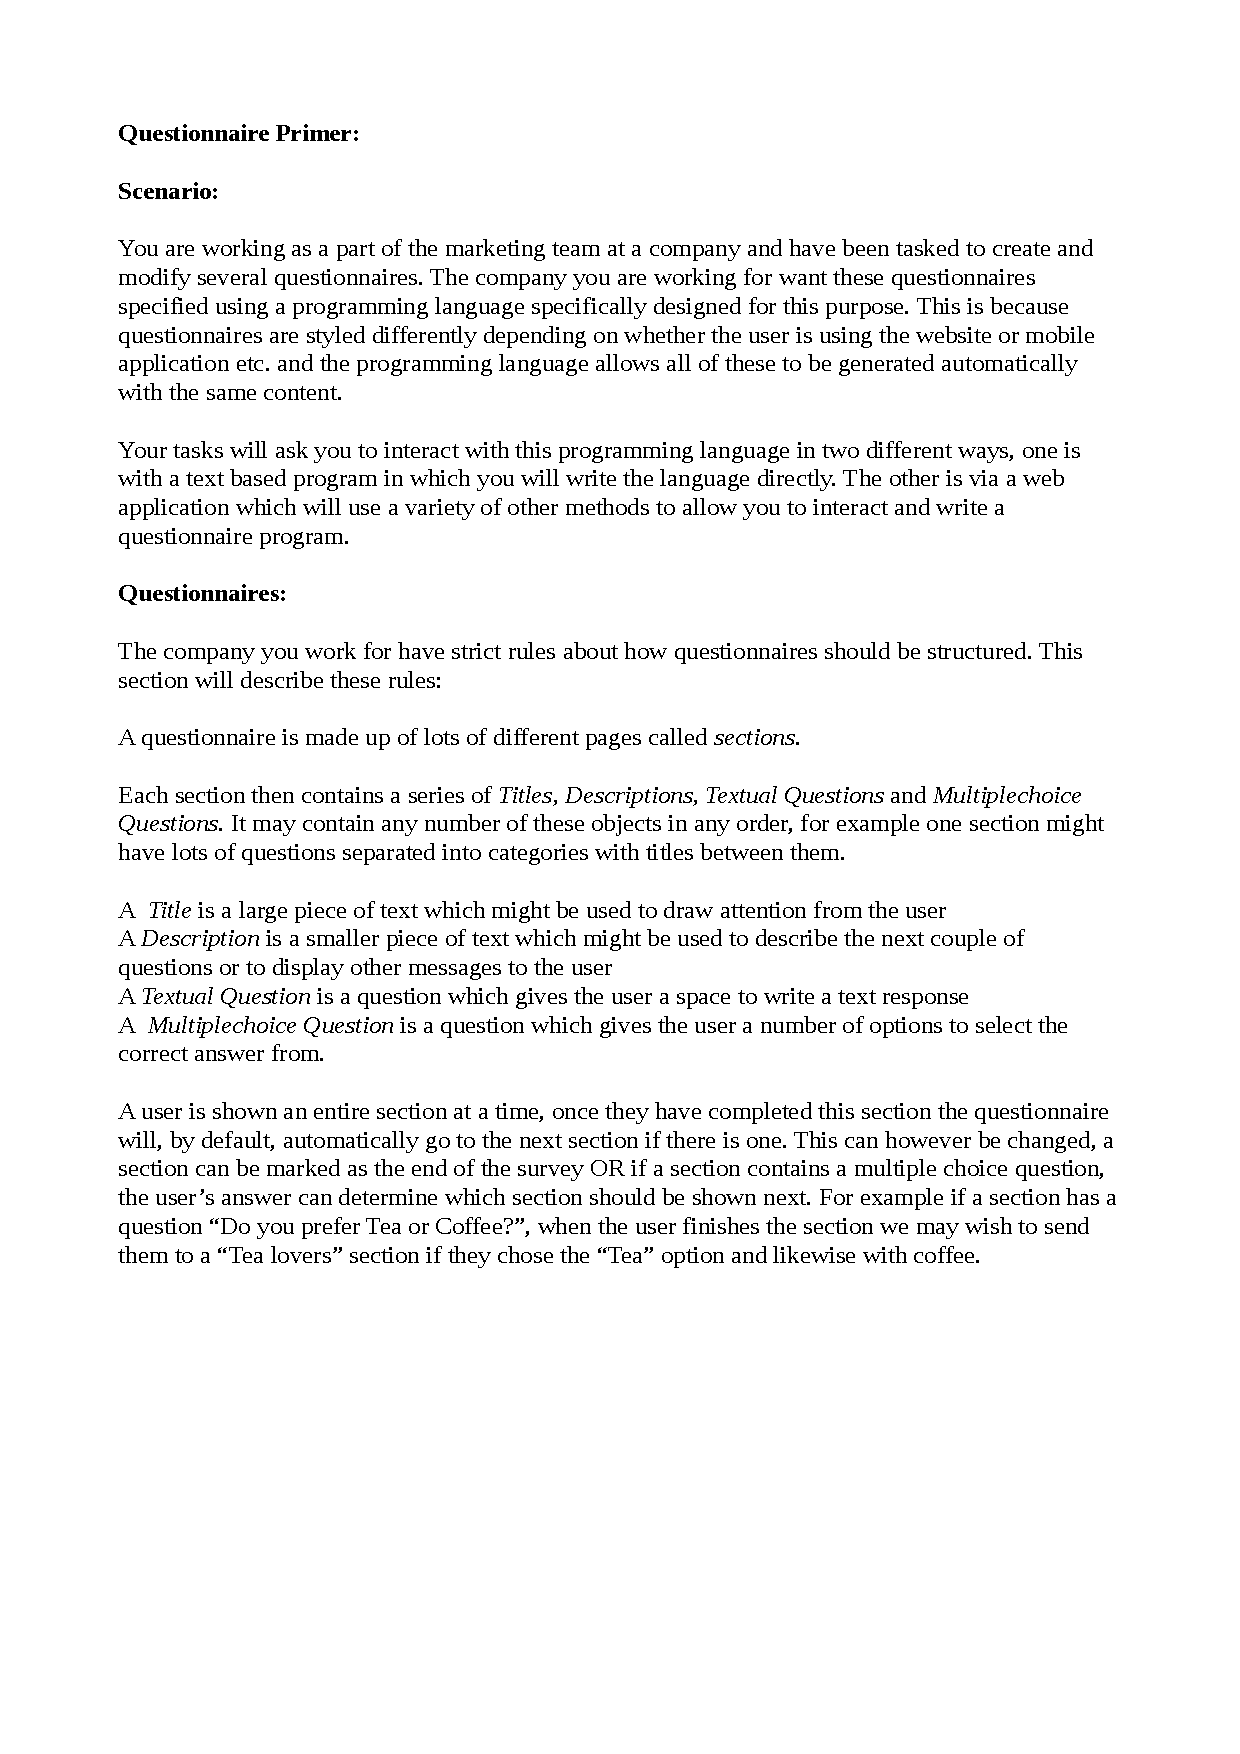
\includepdf[pages=1,scale=.75,pagecommand=\section{Questionnaire Evaluation Materials}\label{questionnaireEval} \subsection{Training Material}]{./Appendix/QuestionnaireTraining.pdf}
\includepdf[pages=2-,scale=.8]{./Appendix/QuestionnaireTraining.pdf}

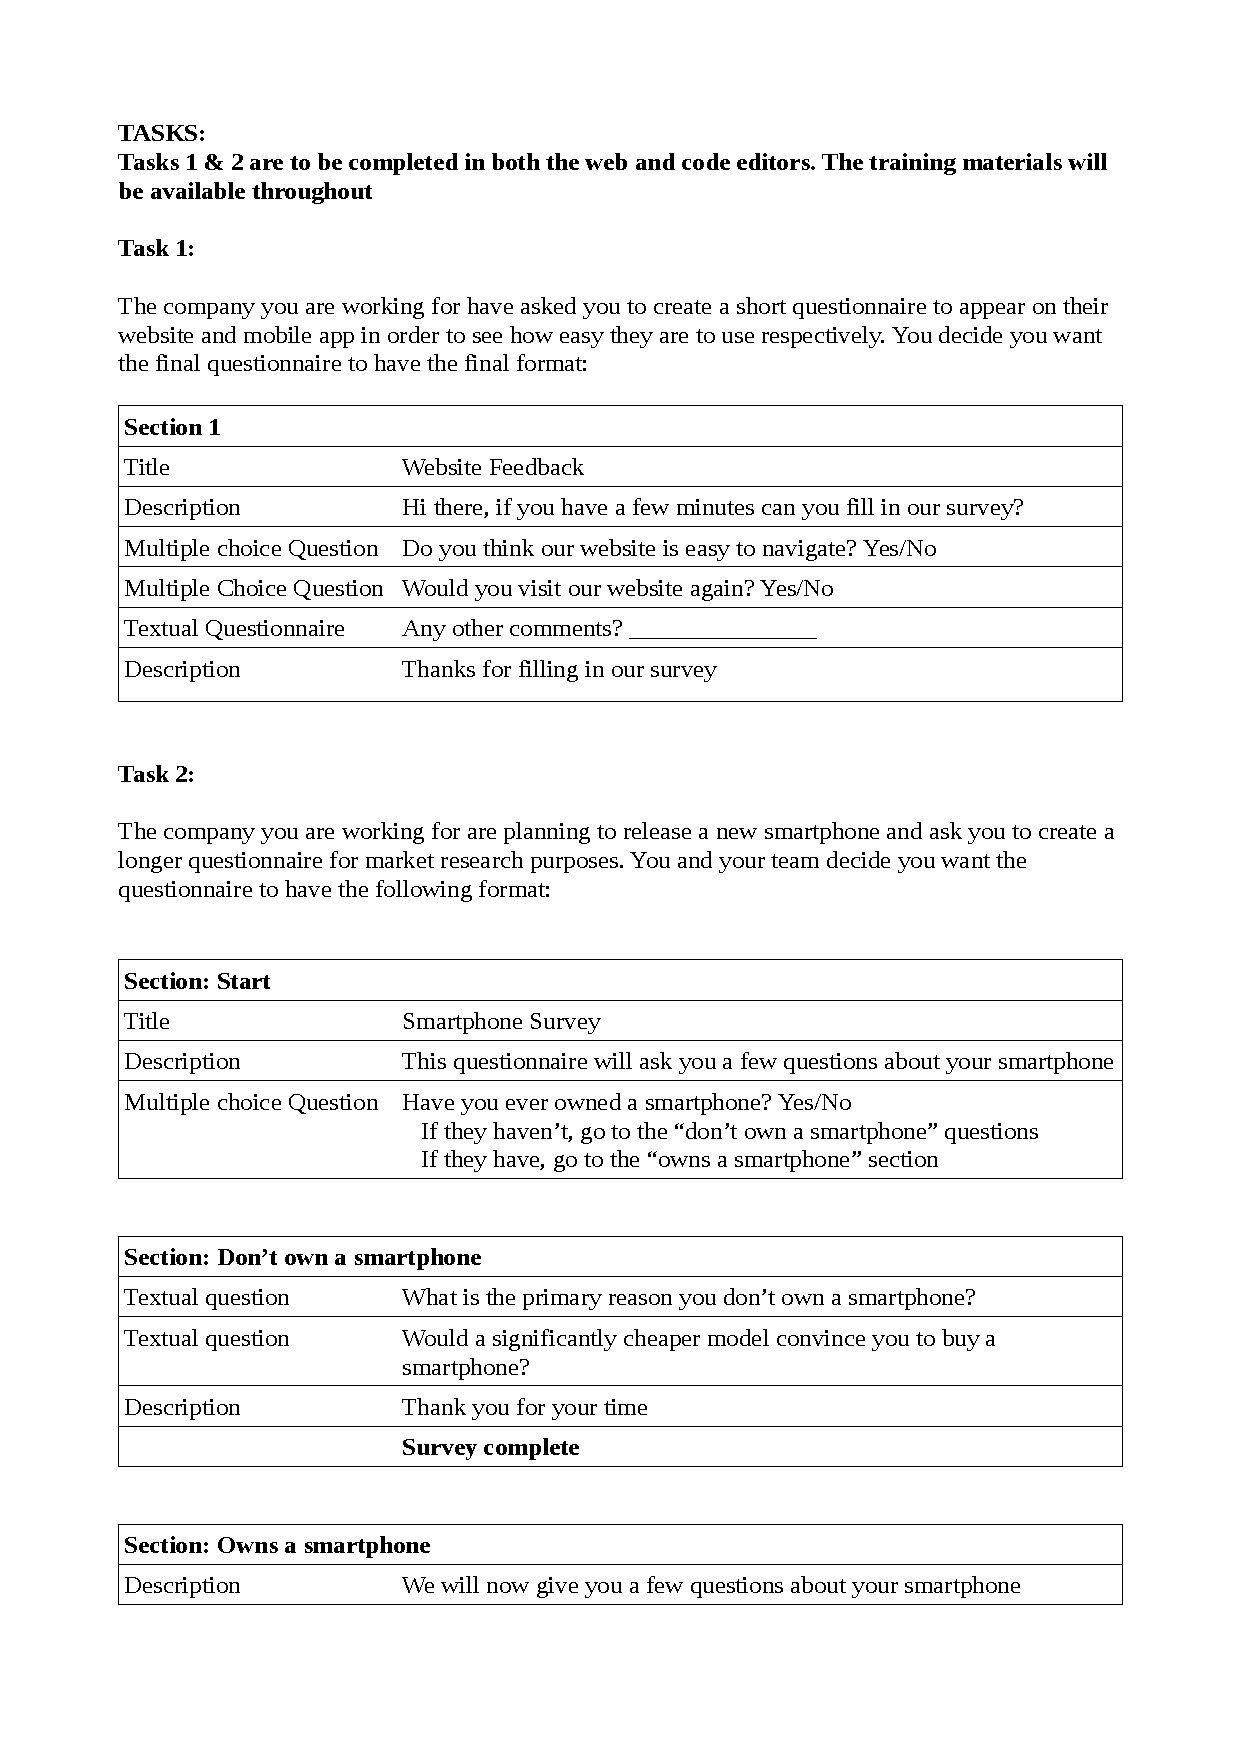
\includepdf[pages=1,scale=.8,pagecommand=\subsection{Task Sheet}]{./Appendix/QuestionnaireTasks.pdf}
\includepdf[pages=2-,scale=.8]{./Appendix/QuestionnaireTasks.pdf}

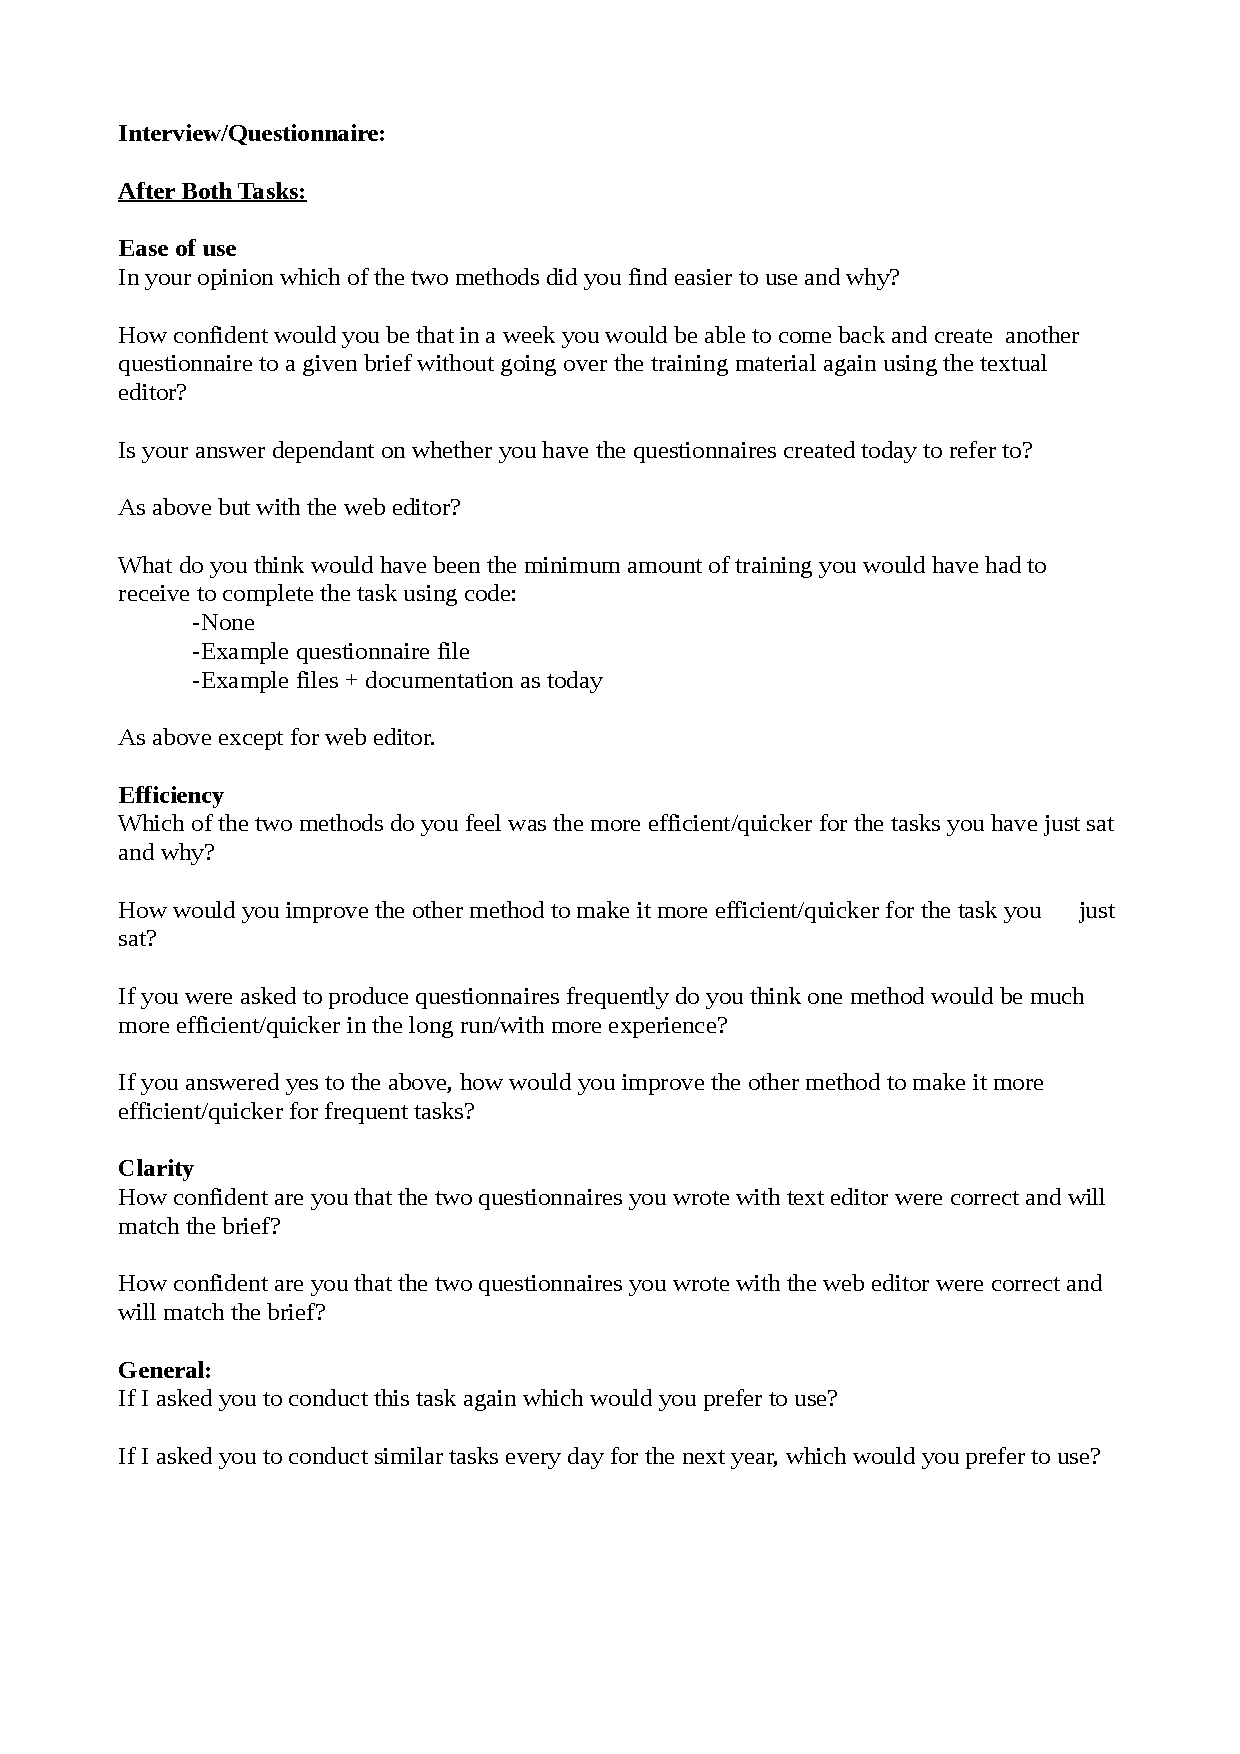
\includepdf[pages=-,scale=.8,pagecommand=\subsection{Interview Questions}]{./Appendix/InterviewQuestions.pdf}

\section{Questionnaire Evaluation Results}\label{questionnaireEvalResults}

\subsection{Respondent 1}
\subsubsection*{First editor used to complete tasks:} Eclipse
\subsubsection*{Times:}
\begin{itemize}
\item \emph{Eclipse Task 1:} 7:28
\item \emph{Eclipse Task 2:} 19:36
\item \emph{Web Task 1:} 2:35
\item \emph{Web Task 2:} 10:25
\end{itemize}
\subsubsection*{Observations made as completing tasks:}

\emph{Eclipse:}
\begin{itemize}
\item Significant confusion caused by curly brace positioning
\item Worried about spacing and initially spent a lot of time trying to perfectly match spaces in example/ training documentation
\item Missed string quotation marks
\item Found the error reporting in Eclipse difficult to deal with, despite positioning of red lines struggled to find where actual error was
\item Confusion from poorly named sections
\item Didn't make use of copy/paste in Android/iPhone section of 2nd task
\item Required help to finish task 2, couldn't work out brace positioning
\end{itemize}
\emph{Web Editor:}
\begin{itemize}
\item Didn't find adding extra sections intuitive, didn't understand how to find section editor and had to ask for help
\item Tried to click on reference to section in main questionnaire view as if it were a link
\item Tried adding goto's to sections that didn't yet exist
\end{itemize}

\subsubsection*{Post Tasks Interview Transcript:}
\textit{In your opinion which of the two methods was the easier to use with the training that you had and why was that? } \\
\\
Definitely the second one
\\
\\
\textit{The web editor?}
\\
\\
Yep.Because having dropdowns made [input easier], you just had to recognise what section to put in as opposed to having to memorise exactly what to type so you just have to be familiar with it as opposed to knowing exactly what to enter. Also not having to put in the brackets in the right places was a massive help.
\\
\\
\textit{If I were to ask you to come again in a weeks time and I were to ask you to create another questionnaire to a given brief but didn't give you the training materials, how confident would you be creating that firstly with the textual editor?}
\\
\\
I'm not even sure I'd be able to create it now, without any errors.
\\
\\
\textit{Would your answer change if you had your previous questionnaires to refer back to so you could see how you'd done things before}\\
\\
No, because even with the training materials today the chances of getting an error were relatively high and the error messages given on the screen weren't terribly intuitive I felt.
\\
\\
\textit{And with the second method [web editor], the same question. If you were to come back in a week and I gave you a questionnaire specification without the training materials, do you think you'd be able to create it from scratch?}
\\
\\
Probably. Yes. I think so yes, it might be a bit slower, but yeh I think I could do it again.
\\
\\
\textit{would you need these examples that you've just created to refer to?}
\\
\\
Probably not, no.
\\
\\
\textit{Efficiency is the next thing we'll talk about. Which of the two methods did you think was quicker?}
\\
\\
The second one. [Web editor] 
\\
\\
\textit{Why did you think that?}
\\
\\
There was less thinking time for me as all the text you have to input wasn't at the front of my brain and so it was a slower process to recall it as I wasn't familiar with it and so that was a bit of a slower process whereas the [web editor] you just had to recognise it so it's much quicker. Also selecting from a drop down is inherently quicker.
\\
\\
\textit{If I were to force you to use the textual editor, how would you make it quicker for you and more efficient?}
\\
\\
Get rid of all the brackets
\\
\\
\textit{So actually changing the language itself?}
\\
\\
Yes, or introduce software that puts them in automatically. As with the Answers surely it's the case that they always have to have those so you could automatically install those. Or have clearer error messages saying where you have to put one.
\\
\\
\textit{If you were to produce these questionnaires really frequently, and you had much more experience with both methods, do you think that would change your answer? Do you think you would still be quicker with the web editor or do you think you would get used to the language to a point where you'd be quicker with that?}
\\
\\
No I think it'd still be quicker with the web editor, but obviously you'd get quicker with the text editor too I think I'd still be faster with the web editor.
\\
\\
\textit{How confident were you that the questionnaires you wrote with the text editor matched the specification?}
\\
\\
Well, apart from the errors which meant it wouldn't have run at all, once those had been corrected I guess relatively confident. I don't know, I've never seen one of these run so I don't know.
\\
\\
\textit{And what about with the web editor?}
\\
\\
Well, because I selected everything from dropdowns in the editor I assume that selecting those options would produce like the website correctly.
\\
\\
\textit{Sorry, I'm asking here not whether or not it'd be able to do the conversion, but whether you think the specification that you typed matches the one given. Does that make sense?}
\\
\\
Yep. Relatively confident, I think. It was quite clear by going back to the questionnaire which sections you had, which I think helps.
\\
\\
\textit{So in general if I were to ask you to do this task again which would you use?}
\\
\\
The web editor.
\\
\\
\textit{And if I were to ask you to do it every day for a year, does that change your opinion?}
\\
\\
I do wonder if selecting drop downs might be more boring, but it is more efficient. But then if this were my job I'd probably be bored either way, so web editor.
\subsection{Respondent 2}
\subsubsection*{First editor used to complete tasks:} Eclipse
\subsubsection*{Times:}
\begin{itemize}
\item \emph{Eclipse Task 1:} 4:24
\item \emph{Eclipse Task 2:} 17:05
\item \emph{Web Task 1:} 3:30
\item \emph{Web Task 2:} 11:03
\end{itemize}
\subsubsection*{Observations made as completing tasks:}

\emph{Eclipse:}
\begin{itemize}
\item Spent significant time during training looking at example file
\item Made use of copy and paste functionality to take structure from example file and modify the relevant fields
\item Unsure about spacing and asked several times if mattered
\item Struggled with curly braces
\item Made use of copy and paste within second task on Android/iPhone sections
\item Missed a curly brace. Despite error underlining where it should be added and error message "Missing '\{'' " respondent assumed issue was elsewhere in the file and to do with spacing. Took sometime to spot real cause
\end{itemize}
\emph{Web Editor:}
\begin{itemize}
\item Found confusing had to add section before could cross reference
\item Did use the sub tree views to modify just a particular question
\end{itemize}

\subsubsection*{Post Tasks Interview Transcript:}

\textit{First question is which of the two methods did you find easier to use and why?}
\\
\\
In terms of actual use in terms of which was more intuitive to work out, the web based one. The web based editor. Although as I got more used to the Eclipse editor that became easier and quicker to use because when the surveys got more repetitive it was easier to just copy and paste and also to change things retrospectively.
\\
\\
\textit{If I were to ask you to come back in a week and write another questionnaire, how confident would you be that you'd be able to do that? Firstly in the web editor, without the training materials.}
\\
\\
Far easier than the text editor. As said it was far more intuitive
\\
\\
\textit{And what about with the Eclipse editor?}
\\
\\
I think with the Eclipse, perhaps if I had the example coding but writing it completely from scratch would be a lot more difficult.
\\
\\
\textit{So you think if you had the example code you would be able to do that, using one of the files you wrote today say to refamiliarise yourself?}
\\
\\
If all the necesary sections were there, then yes. If there were other things that I hadn't been taught then the web based editor would be easier.
\\
\\
\textit{And with the textual, Eclipse editor what do you think the minimal amount of training you would have had to receive? If I'd have sent you an exisiting questionnaire and then a task do you think you could have worked out how to write a specification from the example?}
\\
\\
I believe so yes,but I think if it's the kind of thing you'd keep coming back and forth from, it'd still take a lit of time to relearn it unless you were consistently coding.
\\
\\
\textit{And what about the web editor, do you think you could have used that without any of the documentation you received today?}
\\
\\
Yes I think so, at least with the example questionnaire to map it. Particularly if it was something you could map in advance as you add sections in order so as long as you'd planned it in advance and you had an idea of what your questionnaire would look like it's much easier to map and then once that's in place it's not that bad to intuitively put things together.
\\
\\
\textit{I'm now going to ask you some questions about the efficiency of the two methods. Firstly, which of the two methods do you think was quicker/more efficient, using the terms interchangeably here. For the task that you've just sat, and why?}                                                                                                                                                                                                                                                                \\
\\
I think initially the web based editor was more efficient, but once you'd got to grips with what Eclipse was asking for that became quicker as the tasks progressed. I certainly found answering task 1 easier on the web page than task 1 on Eclipse. But then once you'd kind of got used to it, especially with example code to copy and paste I found that was more efficient.
\\
\\
\textit{How would you improve the web editor then to make it more efficient?}
\\
\\
I think the ability to move sections around and actually be able to edit and duplicate sections. Like the last function on Android or iPhone they are asking for the same thing mapped in the same way and that was easy to copy and paste in the text editor and if you could do that in the web editor that would make things easier. Also if someone were proficient in not necessarily coding but questionnaires or whatever it is they're mapping, if there's not a set plan there should be more room for them to change things as they're doing it. I'm not sure how that manifests itself with this tree, maybe some kind of flowchart where they could move things around. But I think that would make it more intuitive for the purpose of making. Since I think the whole point of this is to make things easier.
\\
\\
\textit{If I were to ask you to produce these questionnaires frequently do you think in the long run one method would be more efficient?}
\\
\\
With more experience I think I'd become more proficient at the code based [Eclipse editor] but if you implemented the changes to make the [web based] more free flowing I think that would be easier in the long run. Even if someone is proficient at coding there is still the risk of human error when you're producing stuff with code as opposed to being funnelled through the web page program.
\\
\\
\textit{If I were to give you a questionnaire written by someone else, that had an issue with it, with specification, such as a spelling mistake or being taken to the wrong section. Which of the two methods would yuou prefer to find that mistake?}
\\
\\
I'd say in that case the text based as you can have all the code in front of you and have an open plan of everything I think the web based is more efficient at times since it funnels you into stuff but if theres a clear problem you have to open every step to look for it.
\\
\\
\textit{If we were to change the web based program to display everything and you had the option to narrow down only if you wanted to, would that change your answer?}
\\
\\
Yes if you added a checkbox on the tree to show all to explode the view that would be very useful and would have all the benefits of the text based editor.
\\
\\
\textit{If I were to ask you to create another survey right now, which of the two methods would you use?}
\\
\\
If it was utilising all the same methods as previously done in the first two tasks I would go for the text based because if the code were in front of me I could copy and paste the layout. If there were anything new or new functions I think the web based would be more efficient
\\
\\
\textit{If I were to ask you to create another survey every day for a year, does your answer change?}
\\
\\
Probably wouldn't change, but if you implemented the changes I suggested that would probably be more efficient.
                                                                                                                                                                                                                                                                                                                                                                                                                                                                                                                                                                                                                                                                                                                                                                                                                                                                                                                                                                                                                                                                                                                                                                                                                                                                                                                                                                                                                                                                                                                                                                                                                                                                                                                                                                                                                                                                                                                                                                                                                                                                                                                                                                                                                                                                                                                                                                                                                                                                                                                                                                                                                                                                                                                                                                                                                                                                                                                                                                                                                                                                                                                                                                                                                                                                                                                                                                                                                                                                                                                                                                                                                                                                                                                                                                                                                                                                                                                                                                                                                                                                                                                                                                                                                                                                                                                                                                                                                                                                                                                                                                                                                                                                                                                                                                                                                                                                          

\subsection{Respondent 3}
\subsubsection*{First editor used to complete tasks:} Web
\subsubsection*{Times:}
\begin{itemize}
\item \emph{Eclipse Task 1:} 4:03
\item \emph{Eclipse Task 2:} 15:14
\item \emph{Web Task 1:} 3:19
\item \emph{Web Task 2:} 10:57
\end{itemize}
\subsubsection*{Observations made as completing tasks:}

\emph{Eclipse:}
\begin{itemize}
\item Missed 'Section' keyword when creating first section in task 1 and had some difficulty in realising this was the cause of an error as the produced error message wasn't clear. Saying only "EOF was expected"
\item Made use of copy and paste on individual questions, modifying relevant attributes only
\item Had little issue with curly braces, perhaps as made use of Eclipse's automatic insertion of these
\end{itemize}
\emph{Web Editor:}
\begin{itemize}
\item Struggled with navigating between questionnaire editor and section editor at first
\item Confusion caused by adding nodes which are generated from the parse tree but in themselves are meaningless, normally only used for other nodes to inherit
\item Tried clicking on references in questionnaire editor
\item Tried adding references in goto feature despite references not yet existing.
\end{itemize}

\subsubsection*{Post Tasks Interview Transcript:}
\textit{Which of the two methods did you find the easier to use?}
\\
\\
The web editor
\\
\\
\textit{And why was that?}
\\
\\
Found it easier to organise and picture what I was doing with graphics rather than text
\\
\\
\textit{If I were to ask you to come back in a week and write a 3rd questionnaire how confident would you be that you'd be able to code that up with Eclipse, without the training materials?}
\\
\\
Without instructions I wouldn't be that confident.
\\
\\
\textit{Would your answer change if you had the ones today to look back on?}
\\
\\
Yeh if I had the ones from today I could do it again.\\
\\
\textit{What about with the web editor?}
\\
\\
I think I could do it.
\\
\\
\textit{Without any example files?}
\\
\\
Yeh
\\
\\
\textit{What is the minimum amount of training you think you'd need to be able to use these editors? Firstly with the Eclipse editor, do you think you could have completed the tasks using just an example file or even nothing at all?}
\\
\\
No, I don't think I would have been able to I needed the instructions.
\\
\\
\textit{What about with the web editor?}
\\
\\
Yeh I probably would have been able to work it out, maybe with a bit of trial and error.
\\
\\
\textit{Which of the two methods did you think was the more efficient, by which I mean quicker?}
\\
\\
I think the web editor was, it's difficult because once I'd already created the survey once it made it easier the second time around but I thought that the web editor was quicker.
\\
\\
\textit{How would you make the Eclipse editor to make it more efficient for the tasks you've just done? Do you think it was missing anything that would have made it easier?}
\\
\\
I just found it slightly difficult to keep track of where the different sections I had created and in visualising it. But I'm not sure how you could improve it from that.
\\
\\
\textit{If I were to ask you to create these questionnaires frequently do you think your answer as to which was more efficient would change given more experience?}
\\
\\
No, there's not really any benefit from the text editor that I'd get having used it more. I don't know, I don't think they'd change much.
\\
\\
\textit{Is there anyway you could improve it either method to make them more efficient in the long run}
\\
\\
I can't think of anything.
\\
\\
\textit{The company you work for come back to you with a questionnaire and they said that there is an issue with it. Something like the sections are out of order or a spelling mistake was present. Which editor do you think would make it easier to find the mistake?}
\\
\\
I suppose the web editor, there's less going on. It'd probably be quite close as the text editor [Eclipse] did give some warnings that pop up. But you have fewer things on your screen with the web editor.
\\
\\
\textit{If I were to ask you to do this task again which would you prefer to use?}
\\
\\
The web editor
\\
\\
\textit{And if I were to ask you to do this again every day for a year which would you prefer to use?}
\\
\\
Web editor


\subsection{Respondent 4}
\subsubsection*{First editor used to complete tasks:} Web
\subsubsection*{Times:}
\begin{itemize}
\item \emph{Eclipse Task 1:} 5:58
\item \emph{Eclipse Task 2:} 17:54
\item \emph{Web Task 1:} 4:43
\item \emph{Web Task 2:} 11:04
\end{itemize}
\subsubsection*{Observations made as completing tasks:}

\emph{Eclipse:}
\begin{itemize}
\item Had to be shown where the curly braces were on a keyboard
\item Didn't use curly braces at one point with a multiple choice question, read error "Need \{ at Answer" which ellicited a "What?" response. Had to spend some time comparing with example file before understood.
\item Surprised by the automatic insertion of "\}" which caused some initial confusion
\item Missed quotation marks around strings in titles and questions to begin with, visibly frustrated by the error which appeared. "What's wrong now!"
\item Was worried about spacing and tried to copy that of example exactly initially 
\end{itemize}
\emph{Web Editor:}
\begin{itemize}
\item Struggled to navigate tree to find the section editor, during both tasks. 
\item First attempted to add section references in goto before they had been added. Once discovered couldn't do this left all goto statements to fill in at end of the task
\item When filling in goto's at end of task found it very difficult to navigate to individual sections as name wasn't in tree
\end{itemize}

\subsubsection*{Post Tasks Interview Transcript:}
\textit{In your opinion which of the two methods was easier to use?}
\\
\\
The first one
\\
\\
\textit{The web editor?}
\\
\\
Yes
\\
\\
\textit{Why was that?}
\\
\\
it was more intuitive and involved less typing
\\
\\
\textit{What was it about the typing that you found difficult then?}
\\
\\
So not necessarily the typing but remembering which extra symbols I needed to include and at which points like the brackets and the quotation marks.
\\
\\
\textit{If I were to come back in a week to create another questionnaire to a different specification, how confident would you be that you'd be able to create that questionnaire using the text editor without the training materials?}
\\
\\
Not at all, I'll have forgotten this by tomorrow.
\\
\\
\textit{What about if you had an example to refer to?}
\\
\\
I think if I had the tasks I just did now to refer to I'd be able to pick it up again, but it would be harder.
\\
\\
\textit{What about with the web based editor?}
\\
\\
That would be easier I don't even think I'd need anything to refer to.
\\
\\
\textit{With the text editor, today you had some documentation and an example file. Do you think you could have done the tasks without either of those things?}
\\
\\
No
\\
\\
\textit{You needed both?}
\\
\\
I needed both, I used both.
\\
\\
\textit{What about with the web editor, could you have done the task without the documentation?}
\\
\\
It was helpful to look at it, but I don't think I would need to look at it again.
\\
\\
\textit{Which of the two methods did you think was the most efficient or quicker?}
\\
\\
The web editor
\\
\\
\textit{And why did you think that?}
\\
\\
Just objectively I think it took less time
\\
\\
\textit{And how would you improve the text editor to make it more efficient?}
\\
\\
I don't know, I don't think you could improve the text editor yourself, you'd just have to get better at it. I mean, if you were to do this everyday you'd get better at it.
\\
\\
\textit{That's actually the next question, so if you were to do these questionnaires frequently do you think one method would be more efficient then?}
\\
\\
So I think you could get as good with the text editor as with the web one but I don't know that, in the long term, one would be more efficent.
\\
\\
\textit{Say I were your boss and I were to come to you with a questionnaire that Jeff wrote and said it had a mistake in it. This mistake definitely lies with the way it's been specified so is either a spelling mistake or sections are in the wrong order. Which method would be easier to find the mistake?}
\\
\\
Web editor.
\\
\\
\textit{And why is that?}
\\
\\
Because with the text editor you'd have to go through the entire text whereas with the web editor you can go into the individual sections and find it more easily.
\\
\\
\textit{And what if you didn't know which section it was in? Say the questionnaire has ten sections in it and a question leads you to the wrong section.}
\\
\\
The text editor then. Actually I don't know, I think it would depend.
\\
\\
\textit{If I were to ask you to create a third survey now which method would you use?}
\\
\\
The web editor
\\
\\
\textit{And if I were to ask you to create one every day for a year which would you use?}
\\
\\
The web editor
\subsection{Respondent 5}
\subsubsection*{First editor used to complete tasks:} Eclipse
\subsubsection*{Times:}
\begin{itemize}
\item \emph{Eclipse Task 1:} 11:01
\item \emph{Eclipse Task 2:} 18:25
\item \emph{Web Task 1:} 3:19
\item \emph{Web Task 2:} 11:42
\end{itemize}
\subsubsection*{Observations made as completing tasks:}

\emph{Eclipse:}
\begin{itemize}
\item Had to be shown where the curly braces were on a keyboard
\item Unsure about spacing in layout of file
\item spaces added to MultipleChoiceQuestion keyword
\item Used example to refer to alot
\item Caught out on one occasion by automatic addition of closing brace by IDE. Found this easily later though
\item Struggled with referencing in the second task alot, added goto reference for section which didn't exist and then as marked as error changed name multiople times, trying to add spacing, quotation marks etc. Until finally realised had to add the section
\end{itemize}
\emph{Web Editor:}
\begin{itemize}
\item Struggled to navigate tree to find the section editor to begin with, although fine after first task
\item Attempted to add section references in goto before they had been added. Once discovered couldn't do this left all goto statements to fill in at end of the task
\end{itemize}

\subsubsection*{Post Tasks Interview Transcript:}
\textit{Which of the two methods was easier to use?}
\\
\\
The second one, the web editor
\\
\\
\textit{And why was that?}
\\
\\
I think having the different options available so you can see how it works and you're less likely to make mistakes in that way as there's a limited amount that can go wrong
\\
\\
\textit{How confident would you be that in a week if I were to ask you to create a questionnaire using the text editor that you'd be able to do it without the training again?}
\\
\\
I probably would be ok, am I allowed the examples?
\\
\\
\textit{Yes}
\\
\\
Then yes probably
\\
\\
\textit{And what if you weren't allowed the examples?}
\\
\\
I think it would take a lot longer, I think I'd get it right eventually but it'd take a while.
\\
\\
\textit{So you think you'd remember how to do it?}
\\
\\
Yes
\\
\\
\textit{What about with the web editor?}
\\
\\
Yes the same I think
\\
\\
\textit{So you think that would be quicker with these [the tasks completed today] to refer to? }
\\
\\
Yes
\\
\\
\textit{With the text editor, what do you think was the minimum amount of training you'd have needed?  Do you think you could have done it without the documentation or without the example file or even without both?}
\\
\\
I think I'd need both
\\
\\
\textit{And with the web editor, do you think you could have done that without documentation?}
\\
\\
No
\\
\\
\textit{Which one did you think was more efficient?}
\\
\\
The web based one
\\
\\
\textit{And why do you think that was the case?}
\\
\\
Maybe because I'd done the other one first which was probably useful. Also the drop down menus meant I didn't have to type everything.
\\
\\
\textit{So how would you improve the textual editor to make it more efficient?}
\\
\\
I don't know. I don't think you could
\\
\\
\textit{If I were to ask you to write these frequently do you think one method would be much better with more experience?}
\\
\\
Yes
\\
\\
\textit{Which one?}
\\
\\
The web based one
\\
\\
\textit{And how would you then improve the textual one to make it more efficient}
\\
\\
I think I'd just have to get more familiar with it. I didn't really know that the crosses meant when something had gone wrong.
\\
\\
\textit{But even with that experience you don't think it would be faster than the web based one?}
\\
\\
No
\\
\\
\textit{If I were to ask you to do the task again now, which would you prefer to use?}
\\
\\
The web editor
\\
\\
\textit{And if I were to ask you to do the same task everyday for a year, which method would you choose if you had to commit to one?}
\\
\\
The web editor

%\end{document}
\end{appendices}
\printbibliography

\end{document}
